

Look again at table \ref{tab:BacteriaStatistics}.
See figure \ref{fig:Boxplot_species}.

\begin{figure*}
    \centering
     \resizebox{\hsize}{!}{%
        % Created by tikzDevice version 0.12.3 on 2019-12-11 20:53:27
% !TEX encoding = UTF-8 Unicode
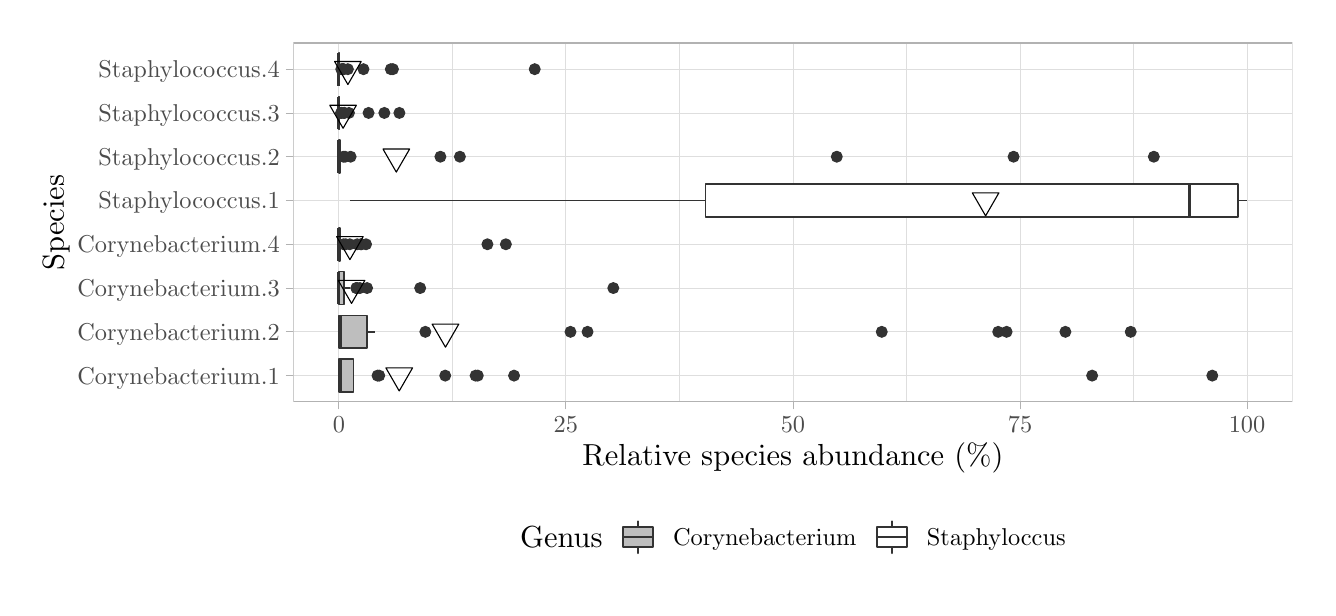
\begin{tikzpicture}[x=1pt,y=1pt]
\definecolor{fillColor}{RGB}{255,255,255}
\path[use as bounding box,fill=fillColor,fill opacity=0.00] (0,0) rectangle (462.53,202.36);
\begin{scope}
\path[clip] (  0.00,  0.00) rectangle (462.53,202.36);
\definecolor{drawColor}{RGB}{255,255,255}
\definecolor{fillColor}{RGB}{255,255,255}

\path[draw=drawColor,line width= 0.6pt,line join=round,line cap=round,fill=fillColor] (  0.00,  0.00) rectangle (462.53,202.36);
\end{scope}
\begin{scope}
\path[clip] ( 96.03, 67.14) rectangle (457.03,196.86);
\definecolor{fillColor}{RGB}{255,255,255}

\path[fill=fillColor] ( 96.03, 67.14) rectangle (457.03,196.86);
\definecolor{drawColor}{gray}{0.87}

\path[draw=drawColor,line width= 0.1pt,line join=round] (153.47, 67.14) --
	(153.47,196.86);

\path[draw=drawColor,line width= 0.1pt,line join=round] (235.51, 67.14) --
	(235.51,196.86);

\path[draw=drawColor,line width= 0.1pt,line join=round] (317.55, 67.14) --
	(317.55,196.86);

\path[draw=drawColor,line width= 0.1pt,line join=round] (399.60, 67.14) --
	(399.60,196.86);

\path[draw=drawColor,line width= 0.3pt,line join=round] ( 96.03, 76.63) --
	(457.03, 76.63);

\path[draw=drawColor,line width= 0.3pt,line join=round] ( 96.03, 92.45) --
	(457.03, 92.45);

\path[draw=drawColor,line width= 0.3pt,line join=round] ( 96.03,108.27) --
	(457.03,108.27);

\path[draw=drawColor,line width= 0.3pt,line join=round] ( 96.03,124.09) --
	(457.03,124.09);

\path[draw=drawColor,line width= 0.3pt,line join=round] ( 96.03,139.91) --
	(457.03,139.91);

\path[draw=drawColor,line width= 0.3pt,line join=round] ( 96.03,155.73) --
	(457.03,155.73);

\path[draw=drawColor,line width= 0.3pt,line join=round] ( 96.03,171.55) --
	(457.03,171.55);

\path[draw=drawColor,line width= 0.3pt,line join=round] ( 96.03,187.36) --
	(457.03,187.36);

\path[draw=drawColor,line width= 0.3pt,line join=round] (112.44, 67.14) --
	(112.44,196.86);

\path[draw=drawColor,line width= 0.3pt,line join=round] (194.49, 67.14) --
	(194.49,196.86);

\path[draw=drawColor,line width= 0.3pt,line join=round] (276.53, 67.14) --
	(276.53,196.86);

\path[draw=drawColor,line width= 0.3pt,line join=round] (358.58, 67.14) --
	(358.58,196.86);

\path[draw=drawColor,line width= 0.3pt,line join=round] (440.62, 67.14) --
	(440.62,196.86);
\definecolor{drawColor}{gray}{0.20}
\definecolor{fillColor}{gray}{0.20}

\path[draw=drawColor,line width= 0.4pt,line join=round,line cap=round,fill=fillColor] (127.04, 76.63) circle (  1.96);

\path[draw=drawColor,line width= 0.4pt,line join=round,line cap=round,fill=fillColor] (126.42, 76.63) circle (  1.96);

\path[draw=drawColor,line width= 0.4pt,line join=round,line cap=round,fill=fillColor] (150.88, 76.63) circle (  1.96);

\path[draw=drawColor,line width= 0.4pt,line join=round,line cap=round,fill=fillColor] (175.75, 76.63) circle (  1.96);

\path[draw=drawColor,line width= 0.4pt,line join=round,line cap=round,fill=fillColor] (162.65, 76.63) circle (  1.96);

\path[draw=drawColor,line width= 0.4pt,line join=round,line cap=round,fill=fillColor] (161.86, 76.63) circle (  1.96);

\path[draw=drawColor,line width= 0.4pt,line join=round,line cap=round,fill=fillColor] (428.06, 76.63) circle (  1.96);

\path[draw=drawColor,line width= 0.4pt,line join=round,line cap=round,fill=fillColor] (384.64, 76.63) circle (  1.96);

\path[draw=drawColor,line width= 0.6pt,line join=round] (117.72, 76.63) -- (118.08, 76.63);

\path[draw=drawColor,line width= 0.6pt,line join=round] (112.44, 76.63) -- (112.44, 76.63);
\definecolor{fillColor}{RGB}{190,190,190}

\path[draw=drawColor,line width= 0.6pt,line join=round,line cap=round,fill=fillColor] (117.72, 70.70) --
	(112.44, 70.70) --
	(112.44, 82.56) --
	(117.72, 82.56) --
	(117.72, 70.70) --
	cycle;

\path[draw=drawColor,line width= 1.1pt,line join=round] (113.09, 70.70) -- (113.09, 82.56);
\definecolor{fillColor}{gray}{0.20}

\path[draw=drawColor,line width= 0.4pt,line join=round,line cap=round,fill=fillColor] (350.69, 92.45) circle (  1.96);

\path[draw=drawColor,line width= 0.4pt,line join=round,line cap=round,fill=fillColor] (374.98, 92.45) circle (  1.96);

\path[draw=drawColor,line width= 0.4pt,line join=round,line cap=round,fill=fillColor] (196.14, 92.45) circle (  1.96);

\path[draw=drawColor,line width= 0.4pt,line join=round,line cap=round,fill=fillColor] (353.73, 92.45) circle (  1.96);

\path[draw=drawColor,line width= 0.4pt,line join=round,line cap=round,fill=fillColor] (143.70, 92.45) circle (  1.96);

\path[draw=drawColor,line width= 0.4pt,line join=round,line cap=round,fill=fillColor] (202.31, 92.45) circle (  1.96);

\path[draw=drawColor,line width= 0.4pt,line join=round,line cap=round,fill=fillColor] (398.58, 92.45) circle (  1.96);

\path[draw=drawColor,line width= 0.4pt,line join=round,line cap=round,fill=fillColor] (308.62, 92.45) circle (  1.96);

\path[draw=drawColor,line width= 0.6pt,line join=round] (122.51, 92.45) -- (125.55, 92.45);

\path[draw=drawColor,line width= 0.6pt,line join=round] (112.44, 92.45) -- (112.44, 92.45);
\definecolor{fillColor}{RGB}{190,190,190}

\path[draw=drawColor,line width= 0.6pt,line join=round,line cap=round,fill=fillColor] (122.51, 86.52) --
	(112.44, 86.52) --
	(112.44, 98.38) --
	(122.51, 98.38) --
	(122.51, 86.52) --
	cycle;

\path[draw=drawColor,line width= 1.1pt,line join=round] (113.10, 86.52) -- (113.10, 98.38);
\definecolor{fillColor}{gray}{0.20}

\path[draw=drawColor,line width= 0.4pt,line join=round,line cap=round,fill=fillColor] (211.62,108.27) circle (  1.96);

\path[draw=drawColor,line width= 0.4pt,line join=round,line cap=round,fill=fillColor] (118.77,108.27) circle (  1.96);

\path[draw=drawColor,line width= 0.4pt,line join=round,line cap=round,fill=fillColor] (118.98,108.27) circle (  1.96);

\path[draw=drawColor,line width= 0.4pt,line join=round,line cap=round,fill=fillColor] (141.83,108.27) circle (  1.96);

\path[draw=drawColor,line width= 0.4pt,line join=round,line cap=round,fill=fillColor] (122.64,108.27) circle (  1.96);

\path[draw=drawColor,line width= 0.4pt,line join=round,line cap=round,fill=fillColor] (118.85,108.27) circle (  1.96);

\path[draw=drawColor,line width= 0.4pt,line join=round,line cap=round,fill=fillColor] (120.07,108.27) circle (  1.96);

\path[draw=drawColor,line width= 0.6pt,line join=round] (114.22,108.27) -- (116.54,108.27);

\path[draw=drawColor,line width= 0.6pt,line join=round] (112.44,108.27) -- (112.44,108.27);
\definecolor{fillColor}{RGB}{190,190,190}

\path[draw=drawColor,line width= 0.6pt,line join=round,line cap=round,fill=fillColor] (114.22,102.34) --
	(112.44,102.34) --
	(112.44,114.20) --
	(114.22,114.20) --
	(114.22,102.34) --
	cycle;

\path[draw=drawColor,line width= 1.1pt,line join=round] (112.44,102.34) -- (112.44,114.20);
\definecolor{fillColor}{gray}{0.20}

\path[draw=drawColor,line width= 0.4pt,line join=round,line cap=round,fill=fillColor] (172.79,124.09) circle (  1.96);

\path[draw=drawColor,line width= 0.4pt,line join=round,line cap=round,fill=fillColor] (114.92,124.09) circle (  1.96);

\path[draw=drawColor,line width= 0.4pt,line join=round,line cap=round,fill=fillColor] (120.37,124.09) circle (  1.96);

\path[draw=drawColor,line width= 0.4pt,line join=round,line cap=round,fill=fillColor] (166.13,124.09) circle (  1.96);

\path[draw=drawColor,line width= 0.4pt,line join=round,line cap=round,fill=fillColor] (116.40,124.09) circle (  1.96);

\path[draw=drawColor,line width= 0.4pt,line join=round,line cap=round,fill=fillColor] (120.60,124.09) circle (  1.96);

\path[draw=drawColor,line width= 0.4pt,line join=round,line cap=round,fill=fillColor] (122.27,124.09) circle (  1.96);

\path[draw=drawColor,line width= 0.4pt,line join=round,line cap=round,fill=fillColor] (114.11,124.09) circle (  1.96);

\path[draw=drawColor,line width= 0.4pt,line join=round,line cap=round,fill=fillColor] (119.07,124.09) circle (  1.96);

\path[draw=drawColor,line width= 0.6pt,line join=round] (112.93,124.09) -- (113.00,124.09);

\path[draw=drawColor,line width= 0.6pt,line join=round] (112.44,124.09) -- (112.44,124.09);
\definecolor{fillColor}{RGB}{190,190,190}

\path[draw=drawColor,line width= 0.6pt,line join=round,line cap=round,fill=fillColor] (112.93,118.16) --
	(112.44,118.16) --
	(112.44,130.02) --
	(112.93,130.02) --
	(112.93,118.16) --
	cycle;

\path[draw=drawColor,line width= 1.1pt,line join=round] (112.44,118.16) -- (112.44,130.02);

\path[draw=drawColor,line width= 0.6pt,line join=round] (437.41,139.91) -- (440.62,139.91);

\path[draw=drawColor,line width= 0.6pt,line join=round] (244.88,139.91) -- (116.39,139.91);
\definecolor{fillColor}{RGB}{255,255,255}

\path[draw=drawColor,line width= 0.6pt,line join=round,line cap=round,fill=fillColor] (437.41,133.98) --
	(244.88,133.98) --
	(244.88,145.84) --
	(437.41,145.84) --
	(437.41,133.98) --
	cycle;

\path[draw=drawColor,line width= 1.1pt,line join=round] (419.86,133.98) -- (419.86,145.84);
\definecolor{fillColor}{gray}{0.20}

\path[draw=drawColor,line width= 0.4pt,line join=round,line cap=round,fill=fillColor] (156.18,155.73) circle (  1.96);

\path[draw=drawColor,line width= 0.4pt,line join=round,line cap=round,fill=fillColor] (292.37,155.73) circle (  1.96);

\path[draw=drawColor,line width= 0.4pt,line join=round,line cap=round,fill=fillColor] (149.14,155.73) circle (  1.96);

\path[draw=drawColor,line width= 0.4pt,line join=round,line cap=round,fill=fillColor] (114.06,155.73) circle (  1.96);

\path[draw=drawColor,line width= 0.4pt,line join=round,line cap=round,fill=fillColor] (116.69,155.73) circle (  1.96);

\path[draw=drawColor,line width= 0.4pt,line join=round,line cap=round,fill=fillColor] (114.71,155.73) circle (  1.96);

\path[draw=drawColor,line width= 0.4pt,line join=round,line cap=round,fill=fillColor] (356.25,155.73) circle (  1.96);

\path[draw=drawColor,line width= 0.4pt,line join=round,line cap=round,fill=fillColor] (406.93,155.73) circle (  1.96);

\path[draw=drawColor,line width= 0.6pt,line join=round] (112.97,155.73) -- (113.69,155.73);

\path[draw=drawColor,line width= 0.6pt,line join=round] (112.44,155.73) -- (112.44,155.73);
\definecolor{fillColor}{RGB}{255,255,255}

\path[draw=drawColor,line width= 0.6pt,line join=round,line cap=round,fill=fillColor] (112.97,149.79) --
	(112.44,149.79) --
	(112.44,161.66) --
	(112.97,161.66) --
	(112.97,149.79) --
	cycle;

\path[draw=drawColor,line width= 1.1pt,line join=round] (112.44,149.79) -- (112.44,161.66);
\definecolor{fillColor}{gray}{0.20}

\path[draw=drawColor,line width= 0.4pt,line join=round,line cap=round,fill=fillColor] (113.41,171.55) circle (  1.96);

\path[draw=drawColor,line width= 0.4pt,line join=round,line cap=round,fill=fillColor] (114.42,171.55) circle (  1.96);

\path[draw=drawColor,line width= 0.4pt,line join=round,line cap=round,fill=fillColor] (128.88,171.55) circle (  1.96);

\path[draw=drawColor,line width= 0.4pt,line join=round,line cap=round,fill=fillColor] (134.32,171.55) circle (  1.96);

\path[draw=drawColor,line width= 0.4pt,line join=round,line cap=round,fill=fillColor] (123.18,171.55) circle (  1.96);

\path[draw=drawColor,line width= 0.4pt,line join=round,line cap=round,fill=fillColor] (114.36,171.55) circle (  1.96);

\path[draw=drawColor,line width= 0.4pt,line join=round,line cap=round,fill=fillColor] (113.21,171.55) circle (  1.96);

\path[draw=drawColor,line width= 0.4pt,line join=round,line cap=round,fill=fillColor] (116.09,171.55) circle (  1.96);

\path[draw=drawColor,line width= 0.6pt,line join=round] (112.66,171.55) -- (112.80,171.55);

\path[draw=drawColor,line width= 0.6pt,line join=round] (112.44,171.55) -- (112.44,171.55);
\definecolor{fillColor}{RGB}{255,255,255}

\path[draw=drawColor,line width= 0.6pt,line join=round,line cap=round,fill=fillColor] (112.66,165.61) --
	(112.44,165.61) --
	(112.44,177.48) --
	(112.66,177.48) --
	(112.66,165.61) --
	cycle;

\path[draw=drawColor,line width= 1.1pt,line join=round] (112.44,165.61) -- (112.44,177.48);
\definecolor{fillColor}{gray}{0.20}

\path[draw=drawColor,line width= 0.4pt,line join=round,line cap=round,fill=fillColor] (114.05,187.36) circle (  1.96);

\path[draw=drawColor,line width= 0.4pt,line join=round,line cap=round,fill=fillColor] (131.22,187.36) circle (  1.96);

\path[draw=drawColor,line width= 0.4pt,line join=round,line cap=round,fill=fillColor] (183.22,187.36) circle (  1.96);

\path[draw=drawColor,line width= 0.4pt,line join=round,line cap=round,fill=fillColor] (114.18,187.36) circle (  1.96);

\path[draw=drawColor,line width= 0.4pt,line join=round,line cap=round,fill=fillColor] (131.99,187.36) circle (  1.96);

\path[draw=drawColor,line width= 0.4pt,line join=round,line cap=round,fill=fillColor] (113.82,187.36) circle (  1.96);

\path[draw=drawColor,line width= 0.4pt,line join=round,line cap=round,fill=fillColor] (121.34,187.36) circle (  1.96);

\path[draw=drawColor,line width= 0.4pt,line join=round,line cap=round,fill=fillColor] (113.31,187.36) circle (  1.96);

\path[draw=drawColor,line width= 0.4pt,line join=round,line cap=round,fill=fillColor] (115.71,187.36) circle (  1.96);

\path[draw=drawColor,line width= 0.6pt,line join=round] (112.73,187.36) -- (112.79,187.36);

\path[draw=drawColor,line width= 0.6pt,line join=round] (112.44,187.36) -- (112.44,187.36);
\definecolor{fillColor}{RGB}{255,255,255}

\path[draw=drawColor,line width= 0.6pt,line join=round,line cap=round,fill=fillColor] (112.73,181.43) --
	(112.44,181.43) --
	(112.44,193.30) --
	(112.73,193.30) --
	(112.73,181.43) --
	cycle;

\path[draw=drawColor,line width= 1.1pt,line join=round] (112.44,181.43) -- (112.44,193.30);
\definecolor{drawColor}{RGB}{0,0,0}

\path[draw=drawColor,line width= 0.4pt,line join=round,line cap=round] (134.26, 71.08) --
	(139.07, 79.41) --
	(129.45, 79.41) --
	(134.26, 71.08);

\path[draw=drawColor,line width= 0.4pt,line join=round,line cap=round] (150.97, 86.90) --
	(155.78, 95.23) --
	(146.16, 95.23) --
	(150.97, 86.90);

\path[draw=drawColor,line width= 0.4pt,line join=round,line cap=round] (117.03,102.72) --
	(121.83,111.04) --
	(112.22,111.04) --
	(117.03,102.72);

\path[draw=drawColor,line width= 0.4pt,line join=round,line cap=round] (116.44,118.54) --
	(121.25,126.86) --
	(111.64,126.86) --
	(116.44,118.54);

\path[draw=drawColor,line width= 0.4pt,line join=round,line cap=round] (346.15,134.36) --
	(350.95,142.68) --
	(341.34,142.68) --
	(346.15,134.36);

\path[draw=drawColor,line width= 0.4pt,line join=round,line cap=round] (133.20,150.18) --
	(138.01,158.50) --
	(128.39,158.50) --
	(133.20,150.18);

\path[draw=drawColor,line width= 0.4pt,line join=round,line cap=round] (113.97,166.00) --
	(118.77,174.32) --
	(109.16,174.32) --
	(113.97,166.00);

\path[draw=drawColor,line width= 0.4pt,line join=round,line cap=round] (115.71,181.81) --
	(120.52,190.14) --
	(110.91,190.14) --
	(115.71,181.81);
\definecolor{drawColor}{gray}{0.70}

\path[draw=drawColor,line width= 0.6pt,line join=round,line cap=round] ( 96.03, 67.14) rectangle (457.03,196.86);
\end{scope}
\begin{scope}
\path[clip] (  0.00,  0.00) rectangle (462.53,202.36);
\definecolor{drawColor}{gray}{0.30}

\node[text=drawColor,anchor=base east,inner sep=0pt, outer sep=0pt, scale=  0.88] at ( 91.08, 73.60) {Corynebacterium.1};

\node[text=drawColor,anchor=base east,inner sep=0pt, outer sep=0pt, scale=  0.88] at ( 91.08, 89.42) {Corynebacterium.2};

\node[text=drawColor,anchor=base east,inner sep=0pt, outer sep=0pt, scale=  0.88] at ( 91.08,105.24) {Corynebacterium.3};

\node[text=drawColor,anchor=base east,inner sep=0pt, outer sep=0pt, scale=  0.88] at ( 91.08,121.06) {Corynebacterium.4};

\node[text=drawColor,anchor=base east,inner sep=0pt, outer sep=0pt, scale=  0.88] at ( 91.08,136.88) {Staphylococcus.1};

\node[text=drawColor,anchor=base east,inner sep=0pt, outer sep=0pt, scale=  0.88] at ( 91.08,152.70) {Staphylococcus.2};

\node[text=drawColor,anchor=base east,inner sep=0pt, outer sep=0pt, scale=  0.88] at ( 91.08,168.52) {Staphylococcus.3};

\node[text=drawColor,anchor=base east,inner sep=0pt, outer sep=0pt, scale=  0.88] at ( 91.08,184.33) {Staphylococcus.4};
\end{scope}
\begin{scope}
\path[clip] (  0.00,  0.00) rectangle (462.53,202.36);
\definecolor{drawColor}{gray}{0.70}

\path[draw=drawColor,line width= 0.3pt,line join=round] ( 93.28, 76.63) --
	( 96.03, 76.63);

\path[draw=drawColor,line width= 0.3pt,line join=round] ( 93.28, 92.45) --
	( 96.03, 92.45);

\path[draw=drawColor,line width= 0.3pt,line join=round] ( 93.28,108.27) --
	( 96.03,108.27);

\path[draw=drawColor,line width= 0.3pt,line join=round] ( 93.28,124.09) --
	( 96.03,124.09);

\path[draw=drawColor,line width= 0.3pt,line join=round] ( 93.28,139.91) --
	( 96.03,139.91);

\path[draw=drawColor,line width= 0.3pt,line join=round] ( 93.28,155.73) --
	( 96.03,155.73);

\path[draw=drawColor,line width= 0.3pt,line join=round] ( 93.28,171.55) --
	( 96.03,171.55);

\path[draw=drawColor,line width= 0.3pt,line join=round] ( 93.28,187.36) --
	( 96.03,187.36);
\end{scope}
\begin{scope}
\path[clip] (  0.00,  0.00) rectangle (462.53,202.36);
\definecolor{drawColor}{gray}{0.70}

\path[draw=drawColor,line width= 0.3pt,line join=round] (112.44, 64.39) --
	(112.44, 67.14);

\path[draw=drawColor,line width= 0.3pt,line join=round] (194.49, 64.39) --
	(194.49, 67.14);

\path[draw=drawColor,line width= 0.3pt,line join=round] (276.53, 64.39) --
	(276.53, 67.14);

\path[draw=drawColor,line width= 0.3pt,line join=round] (358.58, 64.39) --
	(358.58, 67.14);

\path[draw=drawColor,line width= 0.3pt,line join=round] (440.62, 64.39) --
	(440.62, 67.14);
\end{scope}
\begin{scope}
\path[clip] (  0.00,  0.00) rectangle (462.53,202.36);
\definecolor{drawColor}{gray}{0.30}

\node[text=drawColor,anchor=base,inner sep=0pt, outer sep=0pt, scale=  0.88] at (112.44, 56.13) {0};

\node[text=drawColor,anchor=base,inner sep=0pt, outer sep=0pt, scale=  0.88] at (194.49, 56.13) {25};

\node[text=drawColor,anchor=base,inner sep=0pt, outer sep=0pt, scale=  0.88] at (276.53, 56.13) {50};

\node[text=drawColor,anchor=base,inner sep=0pt, outer sep=0pt, scale=  0.88] at (358.58, 56.13) {75};

\node[text=drawColor,anchor=base,inner sep=0pt, outer sep=0pt, scale=  0.88] at (440.62, 56.13) {100};
\end{scope}
\begin{scope}
\path[clip] (  0.00,  0.00) rectangle (462.53,202.36);
\definecolor{drawColor}{RGB}{0,0,0}

\node[text=drawColor,anchor=base,inner sep=0pt, outer sep=0pt, scale=  1.10] at (276.53, 44.09) {Relative species abundance (\%)};
\end{scope}
\begin{scope}
\path[clip] (  0.00,  0.00) rectangle (462.53,202.36);
\definecolor{drawColor}{RGB}{0,0,0}

\node[text=drawColor,rotate= 90.00,anchor=base,inner sep=0pt, outer sep=0pt, scale=  1.10] at ( 13.08,132.00) {Species};
\end{scope}
\begin{scope}
\path[clip] (  0.00,  0.00) rectangle (462.53,202.36);
\definecolor{fillColor}{RGB}{255,255,255}

\path[fill=fillColor] (172.48,  5.50) rectangle (380.58, 30.95);
\end{scope}
\begin{scope}
\path[clip] (  0.00,  0.00) rectangle (462.53,202.36);
\definecolor{drawColor}{RGB}{0,0,0}

\node[text=drawColor,anchor=base west,inner sep=0pt, outer sep=0pt, scale=  1.10] at (177.98, 14.44) {Genus};
\end{scope}
\begin{scope}
\path[clip] (  0.00,  0.00) rectangle (462.53,202.36);
\definecolor{fillColor}{RGB}{255,255,255}

\path[fill=fillColor] (213.25, 11.00) rectangle (227.70, 25.45);
\end{scope}
\begin{scope}
\path[clip] (  0.00,  0.00) rectangle (462.53,202.36);
\definecolor{drawColor}{gray}{0.20}

\path[draw=drawColor,line width= 0.6pt,line join=round,line cap=round] (220.48, 12.45) --
	(220.48, 14.61);

\path[draw=drawColor,line width= 0.6pt,line join=round,line cap=round] (220.48, 21.84) --
	(220.48, 24.01);
\definecolor{fillColor}{RGB}{190,190,190}

\path[draw=drawColor,line width= 0.6pt,line join=round,line cap=round,fill=fillColor] (215.06, 14.61) rectangle (225.90, 21.84);

\path[draw=drawColor,line width= 0.6pt,line join=round,line cap=round] (215.06, 18.23) --
	(225.90, 18.23);
\end{scope}
\begin{scope}
\path[clip] (  0.00,  0.00) rectangle (462.53,202.36);
\definecolor{fillColor}{RGB}{255,255,255}

\path[fill=fillColor] (304.98, 11.00) rectangle (319.43, 25.45);
\end{scope}
\begin{scope}
\path[clip] (  0.00,  0.00) rectangle (462.53,202.36);
\definecolor{drawColor}{gray}{0.20}

\path[draw=drawColor,line width= 0.6pt,line join=round,line cap=round] (312.21, 12.45) --
	(312.21, 14.61);

\path[draw=drawColor,line width= 0.6pt,line join=round,line cap=round] (312.21, 21.84) --
	(312.21, 24.01);
\definecolor{fillColor}{RGB}{255,255,255}

\path[draw=drawColor,line width= 0.6pt,line join=round,line cap=round,fill=fillColor] (306.79, 14.61) rectangle (317.63, 21.84);

\path[draw=drawColor,line width= 0.6pt,line join=round,line cap=round] (306.79, 18.23) --
	(317.63, 18.23);
\end{scope}
\begin{scope}
\path[clip] (  0.00,  0.00) rectangle (462.53,202.36);
\definecolor{drawColor}{RGB}{0,0,0}

\node[text=drawColor,anchor=base west,inner sep=0pt, outer sep=0pt, scale=  0.88] at (233.20, 15.20) {Corynebacterium};
\end{scope}
\begin{scope}
\path[clip] (  0.00,  0.00) rectangle (462.53,202.36);
\definecolor{drawColor}{RGB}{0,0,0}

\node[text=drawColor,anchor=base west,inner sep=0pt, outer sep=0pt, scale=  0.88] at (324.93, 15.20) {Staphyloccus};
\end{scope}
\end{tikzpicture}

    }
    \caption{Boxplots indicating the variation of relative abuncances of different species in the data}
    \label{fig:Boxplot_species}
\end{figure*}

\todo{Paul}{herhalen van theorie in de tekst was eigenlijk specifiek verboden in de opgave. Mag dit wat worden herschreven om de expliciete theorie eruit te laten?}
In the absence of regression the consideration of correlation seems promising to compare the possible associations between the different genus and species. 
The study of the literature revealed that there are basically 3 major correlation methods, 
namely Pearson (r coefficient), Spearman ($\rho$ coefficient) and Kendall ($\tau$ coefficient).
Pearson’s r  is essentially a measure of linearity and requires the data sets to be continuous. 
Moreover, for r to be significant, normality of the data sets is assumed. Which clearly is not the case for the different abundances \todo{all}{(QQ-plots tonen ?)}. 
And if we consider nominal data (the categories of Age for example) Pearson’s r is no longer of use.
Spearman $\rho$ converts the data sets to ranks which are afterwards subjected to a Pearson correlation test to calculate the $\rho$ value. Spearman’s $\rho$ appears to be sensitive to ties in the data, 
which is unfortunately the case in the armpit relative abundances (many zeroes). 
In this case literature points out that Kendall’s $\tau$ is more appropriate as a measure of association. Especially when the number of observations is limited. Kendall’s $\tau$ basically calculates a measure of concordance between couples of data elements from the different sets. 
So for these reasons we opt for the use of Kendall’s $\tau$ measure.
To assert correlation between data sets we need to calculate a p-value for the hypothesis test H0: 
$\tau = 0$ versus Ha: $\tau \neq 0$. If the number of observations is > 10 this can be done by doing a z-test, which we have implemented.
We have also calculated the CI. As the standard R-functions to calculate correlations (such as cor() or cor.test()) do not provide confidence intervals we obtained these through a bootstrapping procedure.

\begin{figure}
    \centering
     \resizebox{\hsize}{!}{%
        % Created by tikzDevice version 0.12.3 on 2019-12-10 19:33:25
% !TEX encoding = UTF-8 Unicode
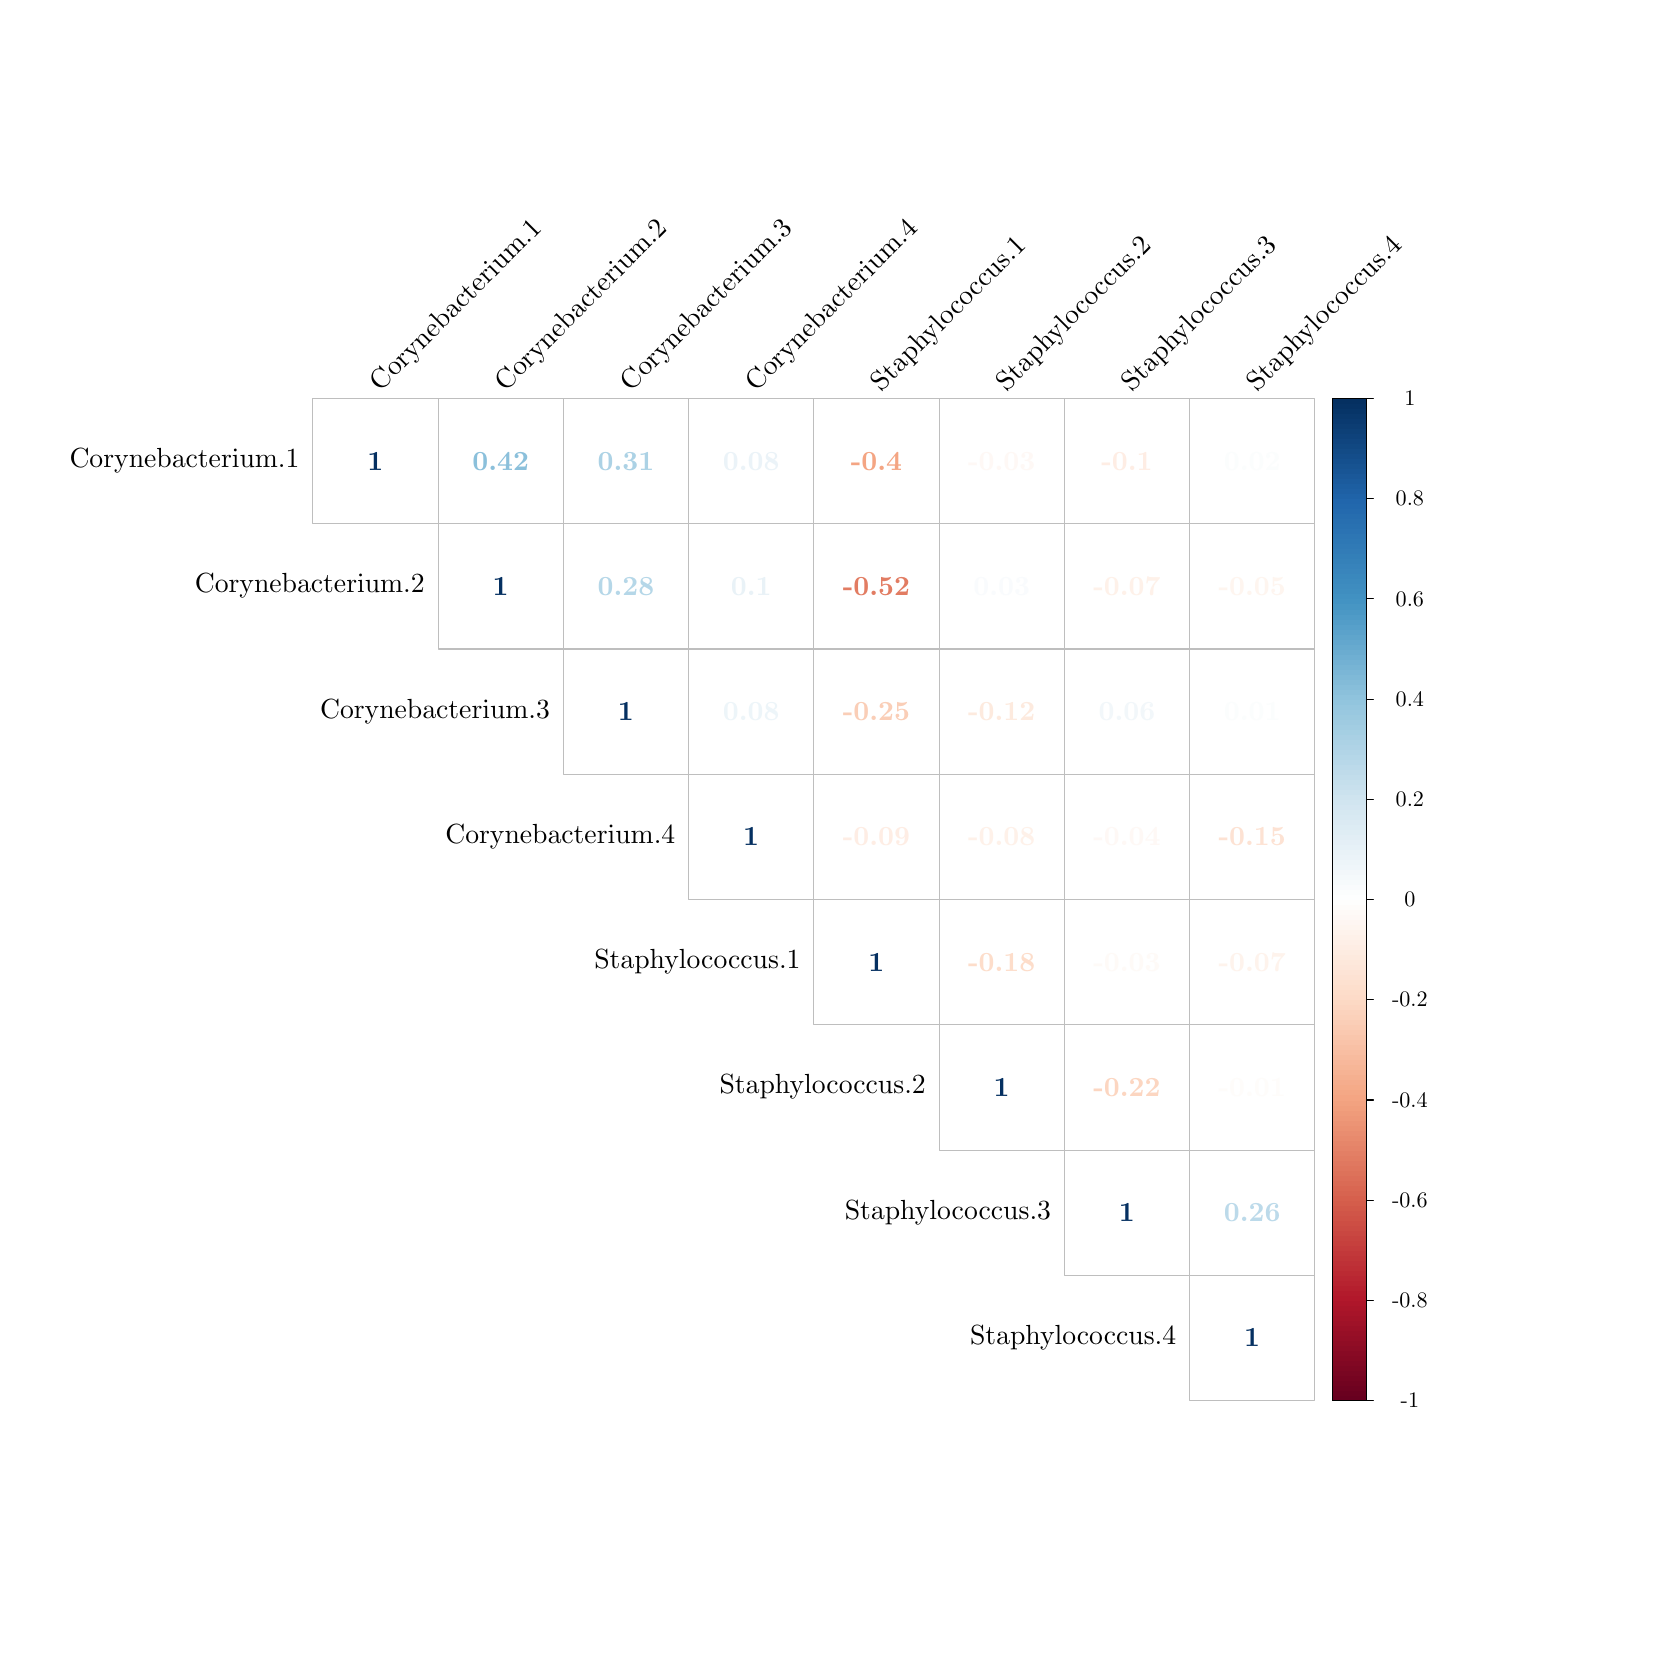
\begin{tikzpicture}[x=1pt,y=1pt]
\definecolor{fillColor}{RGB}{255,255,255}
\path[use as bounding box,fill=fillColor,fill opacity=0.00] (0,0) rectangle (578.16,578.16);
\begin{scope}
\path[clip] (  0.00,  0.00) rectangle (578.16,578.16);
\definecolor{drawColor}{RGB}{255,255,255}
\definecolor{fillColor}{RGB}{255,255,255}

\path[draw=drawColor,line width= 0.4pt,line join=round,line cap=round,fill=fillColor] (103.03,398.88) rectangle (148.29,444.14);

\path[draw=drawColor,line width= 0.4pt,line join=round,line cap=round,fill=fillColor] (148.29,398.88) rectangle (193.55,444.14);

\path[draw=drawColor,line width= 0.4pt,line join=round,line cap=round,fill=fillColor] (148.29,353.62) rectangle (193.55,398.88);

\path[draw=drawColor,line width= 0.4pt,line join=round,line cap=round,fill=fillColor] (193.55,398.88) rectangle (238.81,444.14);

\path[draw=drawColor,line width= 0.4pt,line join=round,line cap=round,fill=fillColor] (193.55,353.62) rectangle (238.81,398.88);

\path[draw=drawColor,line width= 0.4pt,line join=round,line cap=round,fill=fillColor] (193.55,308.36) rectangle (238.81,353.62);

\path[draw=drawColor,line width= 0.4pt,line join=round,line cap=round,fill=fillColor] (238.81,398.88) rectangle (284.07,444.14);

\path[draw=drawColor,line width= 0.4pt,line join=round,line cap=round,fill=fillColor] (238.81,353.62) rectangle (284.07,398.88);

\path[draw=drawColor,line width= 0.4pt,line join=round,line cap=round,fill=fillColor] (238.81,308.36) rectangle (284.07,353.62);

\path[draw=drawColor,line width= 0.4pt,line join=round,line cap=round,fill=fillColor] (238.81,263.10) rectangle (284.07,308.36);

\path[draw=drawColor,line width= 0.4pt,line join=round,line cap=round,fill=fillColor] (284.07,398.88) rectangle (329.33,444.14);

\path[draw=drawColor,line width= 0.4pt,line join=round,line cap=round,fill=fillColor] (284.07,353.62) rectangle (329.33,398.88);

\path[draw=drawColor,line width= 0.4pt,line join=round,line cap=round,fill=fillColor] (284.07,308.36) rectangle (329.33,353.62);

\path[draw=drawColor,line width= 0.4pt,line join=round,line cap=round,fill=fillColor] (284.07,263.10) rectangle (329.33,308.36);

\path[draw=drawColor,line width= 0.4pt,line join=round,line cap=round,fill=fillColor] (284.07,217.84) rectangle (329.33,263.10);

\path[draw=drawColor,line width= 0.4pt,line join=round,line cap=round,fill=fillColor] (329.33,398.88) rectangle (374.59,444.14);

\path[draw=drawColor,line width= 0.4pt,line join=round,line cap=round,fill=fillColor] (329.33,353.62) rectangle (374.59,398.88);

\path[draw=drawColor,line width= 0.4pt,line join=round,line cap=round,fill=fillColor] (329.33,308.36) rectangle (374.59,353.62);

\path[draw=drawColor,line width= 0.4pt,line join=round,line cap=round,fill=fillColor] (329.33,263.10) rectangle (374.59,308.36);

\path[draw=drawColor,line width= 0.4pt,line join=round,line cap=round,fill=fillColor] (329.33,217.84) rectangle (374.59,263.10);

\path[draw=drawColor,line width= 0.4pt,line join=round,line cap=round,fill=fillColor] (329.33,172.58) rectangle (374.59,217.84);

\path[draw=drawColor,line width= 0.4pt,line join=round,line cap=round,fill=fillColor] (374.59,398.88) rectangle (419.84,444.14);

\path[draw=drawColor,line width= 0.4pt,line join=round,line cap=round,fill=fillColor] (374.59,353.62) rectangle (419.84,398.88);

\path[draw=drawColor,line width= 0.4pt,line join=round,line cap=round,fill=fillColor] (374.59,308.36) rectangle (419.84,353.62);

\path[draw=drawColor,line width= 0.4pt,line join=round,line cap=round,fill=fillColor] (374.59,263.10) rectangle (419.84,308.36);

\path[draw=drawColor,line width= 0.4pt,line join=round,line cap=round,fill=fillColor] (374.59,217.84) rectangle (419.84,263.10);

\path[draw=drawColor,line width= 0.4pt,line join=round,line cap=round,fill=fillColor] (374.59,172.58) rectangle (419.84,217.84);

\path[draw=drawColor,line width= 0.4pt,line join=round,line cap=round,fill=fillColor] (374.59,127.32) rectangle (419.84,172.58);

\path[draw=drawColor,line width= 0.4pt,line join=round,line cap=round,fill=fillColor] (419.84,398.88) rectangle (465.10,444.14);

\path[draw=drawColor,line width= 0.4pt,line join=round,line cap=round,fill=fillColor] (419.84,353.62) rectangle (465.10,398.88);

\path[draw=drawColor,line width= 0.4pt,line join=round,line cap=round,fill=fillColor] (419.84,308.36) rectangle (465.10,353.62);

\path[draw=drawColor,line width= 0.4pt,line join=round,line cap=round,fill=fillColor] (419.84,263.10) rectangle (465.10,308.36);

\path[draw=drawColor,line width= 0.4pt,line join=round,line cap=round,fill=fillColor] (419.84,217.84) rectangle (465.10,263.10);

\path[draw=drawColor,line width= 0.4pt,line join=round,line cap=round,fill=fillColor] (419.84,172.58) rectangle (465.10,217.84);

\path[draw=drawColor,line width= 0.4pt,line join=round,line cap=round,fill=fillColor] (419.84,127.32) rectangle (465.10,172.58);

\path[draw=drawColor,line width= 0.4pt,line join=round,line cap=round,fill=fillColor] (419.84, 82.06) rectangle (465.10,127.32);
\definecolor{drawColor}{RGB}{5,48,97}

\node[text=drawColor,anchor=base,inner sep=0pt, outer sep=0pt, scale=  1.00] at (125.66,418.27) {\bfseries 1};
\definecolor{drawColor}{RGB}{139,192,219}

\node[text=drawColor,anchor=base,inner sep=0pt, outer sep=0pt, scale=  1.00] at (170.92,418.27) {\bfseries 0.42};
\definecolor{drawColor}{RGB}{5,48,97}

\node[text=drawColor,anchor=base,inner sep=0pt, outer sep=0pt, scale=  1.00] at (170.92,373.01) {\bfseries 1};
\definecolor{drawColor}{RGB}{172,210,229}

\node[text=drawColor,anchor=base,inner sep=0pt, outer sep=0pt, scale=  1.00] at (216.18,418.27) {\bfseries 0.31};
\definecolor{drawColor}{RGB}{181,215,232}

\node[text=drawColor,anchor=base,inner sep=0pt, outer sep=0pt, scale=  1.00] at (216.18,373.01) {\bfseries 0.28};
\definecolor{drawColor}{RGB}{5,48,97}

\node[text=drawColor,anchor=base,inner sep=0pt, outer sep=0pt, scale=  1.00] at (216.18,327.75) {\bfseries 1};
\definecolor{drawColor}{RGB}{235,243,248}

\node[text=drawColor,anchor=base,inner sep=0pt, outer sep=0pt, scale=  1.00] at (261.44,418.27) {\bfseries 0.08};
\definecolor{drawColor}{RGB}{233,242,247}

\node[text=drawColor,anchor=base,inner sep=0pt, outer sep=0pt, scale=  1.00] at (261.44,373.01) {\bfseries 0.1};
\definecolor{drawColor}{RGB}{237,245,249}

\node[text=drawColor,anchor=base,inner sep=0pt, outer sep=0pt, scale=  1.00] at (261.44,327.75) {\bfseries 0.08};
\definecolor{drawColor}{RGB}{5,48,97}

\node[text=drawColor,anchor=base,inner sep=0pt, outer sep=0pt, scale=  1.00] at (261.44,282.49) {\bfseries 1};
\definecolor{drawColor}{RGB}{244,165,131}

\node[text=drawColor,anchor=base,inner sep=0pt, outer sep=0pt, scale=  1.00] at (306.70,418.27) {\bfseries -0.4};
\definecolor{drawColor}{RGB}{226,124,98}

\node[text=drawColor,anchor=base,inner sep=0pt, outer sep=0pt, scale=  1.00] at (306.70,373.01) {\bfseries -0.52};
\definecolor{drawColor}{RGB}{250,206,183}

\node[text=drawColor,anchor=base,inner sep=0pt, outer sep=0pt, scale=  1.00] at (306.70,327.75) {\bfseries -0.25};
\definecolor{drawColor}{RGB}{254,237,228}

\node[text=drawColor,anchor=base,inner sep=0pt, outer sep=0pt, scale=  1.00] at (306.70,282.49) {\bfseries -0.09};
\definecolor{drawColor}{RGB}{5,48,97}

\node[text=drawColor,anchor=base,inner sep=0pt, outer sep=0pt, scale=  1.00] at (306.70,237.23) {\bfseries 1};
\definecolor{drawColor}{RGB}{254,248,245}

\node[text=drawColor,anchor=base,inner sep=0pt, outer sep=0pt, scale=  1.00] at (351.96,418.27) {\bfseries -0.03};
\definecolor{drawColor}{RGB}{249,251,253}

\node[text=drawColor,anchor=base,inner sep=0pt, outer sep=0pt, scale=  1.00] at (351.96,373.01) {\bfseries 0.03};
\definecolor{drawColor}{RGB}{253,234,222}

\node[text=drawColor,anchor=base,inner sep=0pt, outer sep=0pt, scale=  1.00] at (351.96,327.75) {\bfseries -0.12};
\definecolor{drawColor}{RGB}{254,241,233}

\node[text=drawColor,anchor=base,inner sep=0pt, outer sep=0pt, scale=  1.00] at (351.96,282.49) {\bfseries -0.08};
\definecolor{drawColor}{RGB}{253,221,202}

\node[text=drawColor,anchor=base,inner sep=0pt, outer sep=0pt, scale=  1.00] at (351.96,237.23) {\bfseries -0.18};
\definecolor{drawColor}{RGB}{5,48,97}

\node[text=drawColor,anchor=base,inner sep=0pt, outer sep=0pt, scale=  1.00] at (351.96,191.97) {\bfseries 1};
\definecolor{drawColor}{RGB}{254,237,228}

\node[text=drawColor,anchor=base,inner sep=0pt, outer sep=0pt, scale=  1.00] at (397.21,418.27) {\bfseries -0.1};
\definecolor{drawColor}{RGB}{254,241,233}

\node[text=drawColor,anchor=base,inner sep=0pt, outer sep=0pt, scale=  1.00] at (397.21,373.01) {\bfseries -0.07};
\definecolor{drawColor}{RGB}{242,247,250}

\node[text=drawColor,anchor=base,inner sep=0pt, outer sep=0pt, scale=  1.00] at (397.21,327.75) {\bfseries 0.06};
\definecolor{drawColor}{RGB}{254,248,245}

\node[text=drawColor,anchor=base,inner sep=0pt, outer sep=0pt, scale=  1.00] at (397.21,282.49) {\bfseries -0.04};
\definecolor{drawColor}{RGB}{254,250,247}

\node[text=drawColor,anchor=base,inner sep=0pt, outer sep=0pt, scale=  1.00] at (397.21,237.23) {\bfseries -0.03};
\definecolor{drawColor}{RGB}{252,214,193}

\node[text=drawColor,anchor=base,inner sep=0pt, outer sep=0pt, scale=  1.00] at (397.21,191.97) {\bfseries -0.22};
\definecolor{drawColor}{RGB}{5,48,97}

\node[text=drawColor,anchor=base,inner sep=0pt, outer sep=0pt, scale=  1.00] at (397.21,146.71) {\bfseries 1};
\definecolor{drawColor}{RGB}{251,253,253}

\node[text=drawColor,anchor=base,inner sep=0pt, outer sep=0pt, scale=  1.00] at (442.47,418.27) {\bfseries 0.02};
\definecolor{drawColor}{RGB}{254,245,239}

\node[text=drawColor,anchor=base,inner sep=0pt, outer sep=0pt, scale=  1.00] at (442.47,373.01) {\bfseries -0.05};
\definecolor{drawColor}{RGB}{251,253,253}

\node[text=drawColor,anchor=base,inner sep=0pt, outer sep=0pt, scale=  1.00] at (442.47,327.75) {\bfseries 0.01};
\definecolor{drawColor}{RGB}{253,226,211}

\node[text=drawColor,anchor=base,inner sep=0pt, outer sep=0pt, scale=  1.00] at (442.47,282.49) {\bfseries -0.15};
\definecolor{drawColor}{RGB}{254,243,236}

\node[text=drawColor,anchor=base,inner sep=0pt, outer sep=0pt, scale=  1.00] at (442.47,237.23) {\bfseries -0.07};
\definecolor{drawColor}{RGB}{254,252,250}

\node[text=drawColor,anchor=base,inner sep=0pt, outer sep=0pt, scale=  1.00] at (442.47,191.97) {\bfseries -0.01};
\definecolor{drawColor}{RGB}{188,218,234}

\node[text=drawColor,anchor=base,inner sep=0pt, outer sep=0pt, scale=  1.00] at (442.47,146.71) {\bfseries 0.26};
\definecolor{drawColor}{RGB}{5,48,97}

\node[text=drawColor,anchor=base,inner sep=0pt, outer sep=0pt, scale=  1.00] at (442.47,101.45) {\bfseries 1};
\definecolor{drawColor}{RGB}{190,190,190}

\path[draw=drawColor,line width= 0.4pt,line join=round,line cap=round] (103.03,398.88) rectangle (148.29,444.14);

\path[draw=drawColor,line width= 0.4pt,line join=round,line cap=round] (148.29,398.88) rectangle (193.55,444.14);

\path[draw=drawColor,line width= 0.4pt,line join=round,line cap=round] (148.29,353.62) rectangle (193.55,398.88);

\path[draw=drawColor,line width= 0.4pt,line join=round,line cap=round] (193.55,398.88) rectangle (238.81,444.14);

\path[draw=drawColor,line width= 0.4pt,line join=round,line cap=round] (193.55,353.62) rectangle (238.81,398.88);

\path[draw=drawColor,line width= 0.4pt,line join=round,line cap=round] (193.55,308.36) rectangle (238.81,353.62);

\path[draw=drawColor,line width= 0.4pt,line join=round,line cap=round] (238.81,398.88) rectangle (284.07,444.14);

\path[draw=drawColor,line width= 0.4pt,line join=round,line cap=round] (238.81,353.62) rectangle (284.07,398.88);

\path[draw=drawColor,line width= 0.4pt,line join=round,line cap=round] (238.81,308.36) rectangle (284.07,353.62);

\path[draw=drawColor,line width= 0.4pt,line join=round,line cap=round] (238.81,263.10) rectangle (284.07,308.36);

\path[draw=drawColor,line width= 0.4pt,line join=round,line cap=round] (284.07,398.88) rectangle (329.33,444.14);

\path[draw=drawColor,line width= 0.4pt,line join=round,line cap=round] (284.07,353.62) rectangle (329.33,398.88);

\path[draw=drawColor,line width= 0.4pt,line join=round,line cap=round] (284.07,308.36) rectangle (329.33,353.62);

\path[draw=drawColor,line width= 0.4pt,line join=round,line cap=round] (284.07,263.10) rectangle (329.33,308.36);

\path[draw=drawColor,line width= 0.4pt,line join=round,line cap=round] (284.07,217.84) rectangle (329.33,263.10);

\path[draw=drawColor,line width= 0.4pt,line join=round,line cap=round] (329.33,398.88) rectangle (374.59,444.14);

\path[draw=drawColor,line width= 0.4pt,line join=round,line cap=round] (329.33,353.62) rectangle (374.59,398.88);

\path[draw=drawColor,line width= 0.4pt,line join=round,line cap=round] (329.33,308.36) rectangle (374.59,353.62);

\path[draw=drawColor,line width= 0.4pt,line join=round,line cap=round] (329.33,263.10) rectangle (374.59,308.36);

\path[draw=drawColor,line width= 0.4pt,line join=round,line cap=round] (329.33,217.84) rectangle (374.59,263.10);

\path[draw=drawColor,line width= 0.4pt,line join=round,line cap=round] (329.33,172.58) rectangle (374.59,217.84);

\path[draw=drawColor,line width= 0.4pt,line join=round,line cap=round] (374.59,398.88) rectangle (419.84,444.14);

\path[draw=drawColor,line width= 0.4pt,line join=round,line cap=round] (374.59,353.62) rectangle (419.84,398.88);

\path[draw=drawColor,line width= 0.4pt,line join=round,line cap=round] (374.59,308.36) rectangle (419.84,353.62);

\path[draw=drawColor,line width= 0.4pt,line join=round,line cap=round] (374.59,263.10) rectangle (419.84,308.36);

\path[draw=drawColor,line width= 0.4pt,line join=round,line cap=round] (374.59,217.84) rectangle (419.84,263.10);

\path[draw=drawColor,line width= 0.4pt,line join=round,line cap=round] (374.59,172.58) rectangle (419.84,217.84);

\path[draw=drawColor,line width= 0.4pt,line join=round,line cap=round] (374.59,127.32) rectangle (419.84,172.58);

\path[draw=drawColor,line width= 0.4pt,line join=round,line cap=round] (419.84,398.88) rectangle (465.10,444.14);

\path[draw=drawColor,line width= 0.4pt,line join=round,line cap=round] (419.84,353.62) rectangle (465.10,398.88);

\path[draw=drawColor,line width= 0.4pt,line join=round,line cap=round] (419.84,308.36) rectangle (465.10,353.62);

\path[draw=drawColor,line width= 0.4pt,line join=round,line cap=round] (419.84,263.10) rectangle (465.10,308.36);

\path[draw=drawColor,line width= 0.4pt,line join=round,line cap=round] (419.84,217.84) rectangle (465.10,263.10);

\path[draw=drawColor,line width= 0.4pt,line join=round,line cap=round] (419.84,172.58) rectangle (465.10,217.84);

\path[draw=drawColor,line width= 0.4pt,line join=round,line cap=round] (419.84,127.32) rectangle (465.10,172.58);

\path[draw=drawColor,line width= 0.4pt,line join=round,line cap=round] (419.84, 82.06) rectangle (465.10,127.32);
\definecolor{drawColor}{RGB}{103,0,31}
\definecolor{fillColor}{RGB}{103,0,31}

\path[draw=drawColor,line width= 0.4pt,line join=round,line cap=round,fill=fillColor] (471.44, 82.06) rectangle (483.80, 83.87);
\definecolor{drawColor}{RGB}{106,1,31}
\definecolor{fillColor}{RGB}{106,1,31}

\path[draw=drawColor,line width= 0.4pt,line join=round,line cap=round,fill=fillColor] (471.44, 83.87) rectangle (483.80, 85.68);
\definecolor{drawColor}{RGB}{110,2,32}
\definecolor{fillColor}{RGB}{110,2,32}

\path[draw=drawColor,line width= 0.4pt,line join=round,line cap=round,fill=fillColor] (471.44, 85.68) rectangle (483.80, 87.49);
\definecolor{drawColor}{RGB}{114,3,32}
\definecolor{fillColor}{RGB}{114,3,32}

\path[draw=drawColor,line width= 0.4pt,line join=round,line cap=round,fill=fillColor] (471.44, 87.49) rectangle (483.80, 89.31);
\definecolor{drawColor}{RGB}{118,4,33}
\definecolor{fillColor}{RGB}{118,4,33}

\path[draw=drawColor,line width= 0.4pt,line join=round,line cap=round,fill=fillColor] (471.44, 89.31) rectangle (483.80, 91.12);
\definecolor{drawColor}{RGB}{121,6,34}
\definecolor{fillColor}{RGB}{121,6,34}

\path[draw=drawColor,line width= 0.4pt,line join=round,line cap=round,fill=fillColor] (471.44, 91.12) rectangle (483.80, 92.93);
\definecolor{drawColor}{RGB}{125,7,34}
\definecolor{fillColor}{RGB}{125,7,34}

\path[draw=drawColor,line width= 0.4pt,line join=round,line cap=round,fill=fillColor] (471.44, 92.93) rectangle (483.80, 94.74);
\definecolor{drawColor}{RGB}{129,8,35}
\definecolor{fillColor}{RGB}{129,8,35}

\path[draw=drawColor,line width= 0.4pt,line join=round,line cap=round,fill=fillColor] (471.44, 94.74) rectangle (483.80, 96.55);
\definecolor{drawColor}{RGB}{133,9,35}
\definecolor{fillColor}{RGB}{133,9,35}

\path[draw=drawColor,line width= 0.4pt,line join=round,line cap=round,fill=fillColor] (471.44, 96.55) rectangle (483.80, 98.36);
\definecolor{drawColor}{RGB}{136,10,36}
\definecolor{fillColor}{RGB}{136,10,36}

\path[draw=drawColor,line width= 0.4pt,line join=round,line cap=round,fill=fillColor] (471.44, 98.36) rectangle (483.80,100.17);
\definecolor{drawColor}{RGB}{140,12,37}
\definecolor{fillColor}{RGB}{140,12,37}

\path[draw=drawColor,line width= 0.4pt,line join=round,line cap=round,fill=fillColor] (471.44,100.17) rectangle (483.80,101.98);
\definecolor{drawColor}{RGB}{144,13,37}
\definecolor{fillColor}{RGB}{144,13,37}

\path[draw=drawColor,line width= 0.4pt,line join=round,line cap=round,fill=fillColor] (471.44,101.98) rectangle (483.80,103.79);
\definecolor{drawColor}{RGB}{148,14,38}
\definecolor{fillColor}{RGB}{148,14,38}

\path[draw=drawColor,line width= 0.4pt,line join=round,line cap=round,fill=fillColor] (471.44,103.79) rectangle (483.80,105.60);
\definecolor{drawColor}{RGB}{151,15,38}
\definecolor{fillColor}{RGB}{151,15,38}

\path[draw=drawColor,line width= 0.4pt,line join=round,line cap=round,fill=fillColor] (471.44,105.60) rectangle (483.80,107.41);
\definecolor{drawColor}{RGB}{155,16,39}
\definecolor{fillColor}{RGB}{155,16,39}

\path[draw=drawColor,line width= 0.4pt,line join=round,line cap=round,fill=fillColor] (471.44,107.41) rectangle (483.80,109.22);
\definecolor{drawColor}{RGB}{159,18,40}
\definecolor{fillColor}{RGB}{159,18,40}

\path[draw=drawColor,line width= 0.4pt,line join=round,line cap=round,fill=fillColor] (471.44,109.22) rectangle (483.80,111.03);
\definecolor{drawColor}{RGB}{163,19,40}
\definecolor{fillColor}{RGB}{163,19,40}

\path[draw=drawColor,line width= 0.4pt,line join=round,line cap=round,fill=fillColor] (471.44,111.03) rectangle (483.80,112.84);
\definecolor{drawColor}{RGB}{167,20,41}
\definecolor{fillColor}{RGB}{167,20,41}

\path[draw=drawColor,line width= 0.4pt,line join=round,line cap=round,fill=fillColor] (471.44,112.84) rectangle (483.80,114.65);
\definecolor{drawColor}{RGB}{170,21,41}
\definecolor{fillColor}{RGB}{170,21,41}

\path[draw=drawColor,line width= 0.4pt,line join=round,line cap=round,fill=fillColor] (471.44,114.65) rectangle (483.80,116.46);
\definecolor{drawColor}{RGB}{174,22,42}
\definecolor{fillColor}{RGB}{174,22,42}

\path[draw=drawColor,line width= 0.4pt,line join=round,line cap=round,fill=fillColor] (471.44,116.46) rectangle (483.80,118.27);
\definecolor{drawColor}{RGB}{178,24,43}
\definecolor{fillColor}{RGB}{178,24,43}

\path[draw=drawColor,line width= 0.4pt,line join=round,line cap=round,fill=fillColor] (471.44,118.27) rectangle (483.80,120.08);
\definecolor{drawColor}{RGB}{179,27,44}
\definecolor{fillColor}{RGB}{179,27,44}

\path[draw=drawColor,line width= 0.4pt,line join=round,line cap=round,fill=fillColor] (471.44,120.08) rectangle (483.80,121.89);
\definecolor{drawColor}{RGB}{181,31,46}
\definecolor{fillColor}{RGB}{181,31,46}

\path[draw=drawColor,line width= 0.4pt,line join=round,line cap=round,fill=fillColor] (471.44,121.89) rectangle (483.80,123.70);
\definecolor{drawColor}{RGB}{183,35,48}
\definecolor{fillColor}{RGB}{183,35,48}

\path[draw=drawColor,line width= 0.4pt,line join=round,line cap=round,fill=fillColor] (471.44,123.70) rectangle (483.80,125.51);
\definecolor{drawColor}{RGB}{185,38,50}
\definecolor{fillColor}{RGB}{185,38,50}

\path[draw=drawColor,line width= 0.4pt,line join=round,line cap=round,fill=fillColor] (471.44,125.51) rectangle (483.80,127.32);
\definecolor{drawColor}{RGB}{187,42,51}
\definecolor{fillColor}{RGB}{187,42,51}

\path[draw=drawColor,line width= 0.4pt,line join=round,line cap=round,fill=fillColor] (471.44,127.32) rectangle (483.80,129.13);
\definecolor{drawColor}{RGB}{189,46,53}
\definecolor{fillColor}{RGB}{189,46,53}

\path[draw=drawColor,line width= 0.4pt,line join=round,line cap=round,fill=fillColor] (471.44,129.13) rectangle (483.80,130.94);
\definecolor{drawColor}{RGB}{190,49,55}
\definecolor{fillColor}{RGB}{190,49,55}

\path[draw=drawColor,line width= 0.4pt,line join=round,line cap=round,fill=fillColor] (471.44,130.94) rectangle (483.80,132.75);
\definecolor{drawColor}{RGB}{192,53,56}
\definecolor{fillColor}{RGB}{192,53,56}

\path[draw=drawColor,line width= 0.4pt,line join=round,line cap=round,fill=fillColor] (471.44,132.75) rectangle (483.80,134.56);
\definecolor{drawColor}{RGB}{194,56,58}
\definecolor{fillColor}{RGB}{194,56,58}

\path[draw=drawColor,line width= 0.4pt,line join=round,line cap=round,fill=fillColor] (471.44,134.56) rectangle (483.80,136.38);
\definecolor{drawColor}{RGB}{196,60,60}
\definecolor{fillColor}{RGB}{196,60,60}

\path[draw=drawColor,line width= 0.4pt,line join=round,line cap=round,fill=fillColor] (471.44,136.38) rectangle (483.80,138.19);
\definecolor{drawColor}{RGB}{198,64,61}
\definecolor{fillColor}{RGB}{198,64,61}

\path[draw=drawColor,line width= 0.4pt,line join=round,line cap=round,fill=fillColor] (471.44,138.19) rectangle (483.80,140.00);
\definecolor{drawColor}{RGB}{199,67,63}
\definecolor{fillColor}{RGB}{199,67,63}

\path[draw=drawColor,line width= 0.4pt,line join=round,line cap=round,fill=fillColor] (471.44,140.00) rectangle (483.80,141.81);
\definecolor{drawColor}{RGB}{201,71,65}
\definecolor{fillColor}{RGB}{201,71,65}

\path[draw=drawColor,line width= 0.4pt,line join=round,line cap=round,fill=fillColor] (471.44,141.81) rectangle (483.80,143.62);
\definecolor{drawColor}{RGB}{203,75,67}
\definecolor{fillColor}{RGB}{203,75,67}

\path[draw=drawColor,line width= 0.4pt,line join=round,line cap=round,fill=fillColor] (471.44,143.62) rectangle (483.80,145.43);
\definecolor{drawColor}{RGB}{205,78,68}
\definecolor{fillColor}{RGB}{205,78,68}

\path[draw=drawColor,line width= 0.4pt,line join=round,line cap=round,fill=fillColor] (471.44,145.43) rectangle (483.80,147.24);
\definecolor{drawColor}{RGB}{207,82,70}
\definecolor{fillColor}{RGB}{207,82,70}

\path[draw=drawColor,line width= 0.4pt,line join=round,line cap=round,fill=fillColor] (471.44,147.24) rectangle (483.80,149.05);
\definecolor{drawColor}{RGB}{208,85,72}
\definecolor{fillColor}{RGB}{208,85,72}

\path[draw=drawColor,line width= 0.4pt,line join=round,line cap=round,fill=fillColor] (471.44,149.05) rectangle (483.80,150.86);
\definecolor{drawColor}{RGB}{210,89,73}
\definecolor{fillColor}{RGB}{210,89,73}

\path[draw=drawColor,line width= 0.4pt,line join=round,line cap=round,fill=fillColor] (471.44,150.86) rectangle (483.80,152.67);
\definecolor{drawColor}{RGB}{212,93,75}
\definecolor{fillColor}{RGB}{212,93,75}

\path[draw=drawColor,line width= 0.4pt,line join=round,line cap=round,fill=fillColor] (471.44,152.67) rectangle (483.80,154.48);
\definecolor{drawColor}{RGB}{214,96,77}
\definecolor{fillColor}{RGB}{214,96,77}

\path[draw=drawColor,line width= 0.4pt,line join=round,line cap=round,fill=fillColor] (471.44,154.48) rectangle (483.80,156.29);
\definecolor{drawColor}{RGB}{215,100,80}
\definecolor{fillColor}{RGB}{215,100,80}

\path[draw=drawColor,line width= 0.4pt,line join=round,line cap=round,fill=fillColor] (471.44,156.29) rectangle (483.80,158.10);
\definecolor{drawColor}{RGB}{217,103,82}
\definecolor{fillColor}{RGB}{217,103,82}

\path[draw=drawColor,line width= 0.4pt,line join=round,line cap=round,fill=fillColor] (471.44,158.10) rectangle (483.80,159.91);
\definecolor{drawColor}{RGB}{218,107,85}
\definecolor{fillColor}{RGB}{218,107,85}

\path[draw=drawColor,line width= 0.4pt,line join=round,line cap=round,fill=fillColor] (471.44,159.91) rectangle (483.80,161.72);
\definecolor{drawColor}{RGB}{220,110,88}
\definecolor{fillColor}{RGB}{220,110,88}

\path[draw=drawColor,line width= 0.4pt,line join=round,line cap=round,fill=fillColor] (471.44,161.72) rectangle (483.80,163.53);
\definecolor{drawColor}{RGB}{221,114,90}
\definecolor{fillColor}{RGB}{221,114,90}

\path[draw=drawColor,line width= 0.4pt,line join=round,line cap=round,fill=fillColor] (471.44,163.53) rectangle (483.80,165.34);
\definecolor{drawColor}{RGB}{223,117,93}
\definecolor{fillColor}{RGB}{223,117,93}

\path[draw=drawColor,line width= 0.4pt,line join=round,line cap=round,fill=fillColor] (471.44,165.34) rectangle (483.80,167.15);
\definecolor{drawColor}{RGB}{224,120,96}
\definecolor{fillColor}{RGB}{224,120,96}

\path[draw=drawColor,line width= 0.4pt,line join=round,line cap=round,fill=fillColor] (471.44,167.15) rectangle (483.80,168.96);
\definecolor{drawColor}{RGB}{226,124,98}
\definecolor{fillColor}{RGB}{226,124,98}

\path[draw=drawColor,line width= 0.4pt,line join=round,line cap=round,fill=fillColor] (471.44,168.96) rectangle (483.80,170.77);
\definecolor{drawColor}{RGB}{227,127,101}
\definecolor{fillColor}{RGB}{227,127,101}

\path[draw=drawColor,line width= 0.4pt,line join=round,line cap=round,fill=fillColor] (471.44,170.77) rectangle (483.80,172.58);
\definecolor{drawColor}{RGB}{229,131,104}
\definecolor{fillColor}{RGB}{229,131,104}

\path[draw=drawColor,line width= 0.4pt,line join=round,line cap=round,fill=fillColor] (471.44,172.58) rectangle (483.80,174.39);
\definecolor{drawColor}{RGB}{230,134,106}
\definecolor{fillColor}{RGB}{230,134,106}

\path[draw=drawColor,line width= 0.4pt,line join=round,line cap=round,fill=fillColor] (471.44,174.39) rectangle (483.80,176.20);
\definecolor{drawColor}{RGB}{232,138,109}
\definecolor{fillColor}{RGB}{232,138,109}

\path[draw=drawColor,line width= 0.4pt,line join=round,line cap=round,fill=fillColor] (471.44,176.20) rectangle (483.80,178.01);
\definecolor{drawColor}{RGB}{233,141,112}
\definecolor{fillColor}{RGB}{233,141,112}

\path[draw=drawColor,line width= 0.4pt,line join=round,line cap=round,fill=fillColor] (471.44,178.01) rectangle (483.80,179.82);
\definecolor{drawColor}{RGB}{235,145,114}
\definecolor{fillColor}{RGB}{235,145,114}

\path[draw=drawColor,line width= 0.4pt,line join=round,line cap=round,fill=fillColor] (471.44,179.82) rectangle (483.80,181.64);
\definecolor{drawColor}{RGB}{236,148,117}
\definecolor{fillColor}{RGB}{236,148,117}

\path[draw=drawColor,line width= 0.4pt,line join=round,line cap=round,fill=fillColor] (471.44,181.64) rectangle (483.80,183.45);
\definecolor{drawColor}{RGB}{238,152,120}
\definecolor{fillColor}{RGB}{238,152,120}

\path[draw=drawColor,line width= 0.4pt,line join=round,line cap=round,fill=fillColor] (471.44,183.45) rectangle (483.80,185.26);
\definecolor{drawColor}{RGB}{239,155,122}
\definecolor{fillColor}{RGB}{239,155,122}

\path[draw=drawColor,line width= 0.4pt,line join=round,line cap=round,fill=fillColor] (471.44,185.26) rectangle (483.80,187.07);
\definecolor{drawColor}{RGB}{241,159,125}
\definecolor{fillColor}{RGB}{241,159,125}

\path[draw=drawColor,line width= 0.4pt,line join=round,line cap=round,fill=fillColor] (471.44,187.07) rectangle (483.80,188.88);
\definecolor{drawColor}{RGB}{242,162,128}
\definecolor{fillColor}{RGB}{242,162,128}

\path[draw=drawColor,line width= 0.4pt,line join=round,line cap=round,fill=fillColor] (471.44,188.88) rectangle (483.80,190.69);
\definecolor{drawColor}{RGB}{244,165,131}
\definecolor{fillColor}{RGB}{244,165,131}

\path[draw=drawColor,line width= 0.4pt,line join=round,line cap=round,fill=fillColor] (471.44,190.69) rectangle (483.80,192.50);
\definecolor{drawColor}{RGB}{244,168,134}
\definecolor{fillColor}{RGB}{244,168,134}

\path[draw=drawColor,line width= 0.4pt,line join=round,line cap=round,fill=fillColor] (471.44,192.50) rectangle (483.80,194.31);
\definecolor{drawColor}{RGB}{245,171,137}
\definecolor{fillColor}{RGB}{245,171,137}

\path[draw=drawColor,line width= 0.4pt,line join=round,line cap=round,fill=fillColor] (471.44,194.31) rectangle (483.80,196.12);
\definecolor{drawColor}{RGB}{245,173,141}
\definecolor{fillColor}{RGB}{245,173,141}

\path[draw=drawColor,line width= 0.4pt,line join=round,line cap=round,fill=fillColor] (471.44,196.12) rectangle (483.80,197.93);
\definecolor{drawColor}{RGB}{245,176,144}
\definecolor{fillColor}{RGB}{245,176,144}

\path[draw=drawColor,line width= 0.4pt,line join=round,line cap=round,fill=fillColor] (471.44,197.93) rectangle (483.80,199.74);
\definecolor{drawColor}{RGB}{246,179,148}
\definecolor{fillColor}{RGB}{246,179,148}

\path[draw=drawColor,line width= 0.4pt,line join=round,line cap=round,fill=fillColor] (471.44,199.74) rectangle (483.80,201.55);
\definecolor{drawColor}{RGB}{246,182,151}
\definecolor{fillColor}{RGB}{246,182,151}

\path[draw=drawColor,line width= 0.4pt,line join=round,line cap=round,fill=fillColor] (471.44,201.55) rectangle (483.80,203.36);
\definecolor{drawColor}{RGB}{247,184,155}
\definecolor{fillColor}{RGB}{247,184,155}

\path[draw=drawColor,line width= 0.4pt,line join=round,line cap=round,fill=fillColor] (471.44,203.36) rectangle (483.80,205.17);
\definecolor{drawColor}{RGB}{247,187,158}
\definecolor{fillColor}{RGB}{247,187,158}

\path[draw=drawColor,line width= 0.4pt,line join=round,line cap=round,fill=fillColor] (471.44,205.17) rectangle (483.80,206.98);
\definecolor{drawColor}{RGB}{248,190,162}
\definecolor{fillColor}{RGB}{248,190,162}

\path[draw=drawColor,line width= 0.4pt,line join=round,line cap=round,fill=fillColor] (471.44,206.98) rectangle (483.80,208.79);
\definecolor{drawColor}{RGB}{248,192,165}
\definecolor{fillColor}{RGB}{248,192,165}

\path[draw=drawColor,line width= 0.4pt,line join=round,line cap=round,fill=fillColor] (471.44,208.79) rectangle (483.80,210.60);
\definecolor{drawColor}{RGB}{249,195,169}
\definecolor{fillColor}{RGB}{249,195,169}

\path[draw=drawColor,line width= 0.4pt,line join=round,line cap=round,fill=fillColor] (471.44,210.60) rectangle (483.80,212.41);
\definecolor{drawColor}{RGB}{249,198,172}
\definecolor{fillColor}{RGB}{249,198,172}

\path[draw=drawColor,line width= 0.4pt,line join=round,line cap=round,fill=fillColor] (471.44,212.41) rectangle (483.80,214.22);
\definecolor{drawColor}{RGB}{250,201,176}
\definecolor{fillColor}{RGB}{250,201,176}

\path[draw=drawColor,line width= 0.4pt,line join=round,line cap=round,fill=fillColor] (471.44,214.22) rectangle (483.80,216.03);
\definecolor{drawColor}{RGB}{250,203,179}
\definecolor{fillColor}{RGB}{250,203,179}

\path[draw=drawColor,line width= 0.4pt,line join=round,line cap=round,fill=fillColor] (471.44,216.03) rectangle (483.80,217.84);
\definecolor{drawColor}{RGB}{250,206,183}
\definecolor{fillColor}{RGB}{250,206,183}

\path[draw=drawColor,line width= 0.4pt,line join=round,line cap=round,fill=fillColor] (471.44,217.84) rectangle (483.80,219.65);
\definecolor{drawColor}{RGB}{251,209,186}
\definecolor{fillColor}{RGB}{251,209,186}

\path[draw=drawColor,line width= 0.4pt,line join=round,line cap=round,fill=fillColor] (471.44,219.65) rectangle (483.80,221.46);
\definecolor{drawColor}{RGB}{251,211,189}
\definecolor{fillColor}{RGB}{251,211,189}

\path[draw=drawColor,line width= 0.4pt,line join=round,line cap=round,fill=fillColor] (471.44,221.46) rectangle (483.80,223.27);
\definecolor{drawColor}{RGB}{252,214,193}
\definecolor{fillColor}{RGB}{252,214,193}

\path[draw=drawColor,line width= 0.4pt,line join=round,line cap=round,fill=fillColor] (471.44,223.27) rectangle (483.80,225.08);
\definecolor{drawColor}{RGB}{252,217,196}
\definecolor{fillColor}{RGB}{252,217,196}

\path[draw=drawColor,line width= 0.4pt,line join=round,line cap=round,fill=fillColor] (471.44,225.08) rectangle (483.80,226.89);
\definecolor{drawColor}{RGB}{253,219,200}
\definecolor{fillColor}{RGB}{253,219,200}

\path[draw=drawColor,line width= 0.4pt,line join=round,line cap=round,fill=fillColor] (471.44,226.89) rectangle (483.80,228.71);
\definecolor{drawColor}{RGB}{253,221,202}
\definecolor{fillColor}{RGB}{253,221,202}

\path[draw=drawColor,line width= 0.4pt,line join=round,line cap=round,fill=fillColor] (471.44,228.71) rectangle (483.80,230.52);
\definecolor{drawColor}{RGB}{253,223,205}
\definecolor{fillColor}{RGB}{253,223,205}

\path[draw=drawColor,line width= 0.4pt,line join=round,line cap=round,fill=fillColor] (471.44,230.52) rectangle (483.80,232.33);
\definecolor{drawColor}{RGB}{253,225,208}
\definecolor{fillColor}{RGB}{253,225,208}

\path[draw=drawColor,line width= 0.4pt,line join=round,line cap=round,fill=fillColor] (471.44,232.33) rectangle (483.80,234.14);
\definecolor{drawColor}{RGB}{253,226,211}
\definecolor{fillColor}{RGB}{253,226,211}

\path[draw=drawColor,line width= 0.4pt,line join=round,line cap=round,fill=fillColor] (471.44,234.14) rectangle (483.80,235.95);
\definecolor{drawColor}{RGB}{253,228,214}
\definecolor{fillColor}{RGB}{253,228,214}

\path[draw=drawColor,line width= 0.4pt,line join=round,line cap=round,fill=fillColor] (471.44,235.95) rectangle (483.80,237.76);
\definecolor{drawColor}{RGB}{253,230,217}
\definecolor{fillColor}{RGB}{253,230,217}

\path[draw=drawColor,line width= 0.4pt,line join=round,line cap=round,fill=fillColor] (471.44,237.76) rectangle (483.80,239.57);
\definecolor{drawColor}{RGB}{253,232,219}
\definecolor{fillColor}{RGB}{253,232,219}

\path[draw=drawColor,line width= 0.4pt,line join=round,line cap=round,fill=fillColor] (471.44,239.57) rectangle (483.80,241.38);
\definecolor{drawColor}{RGB}{253,234,222}
\definecolor{fillColor}{RGB}{253,234,222}

\path[draw=drawColor,line width= 0.4pt,line join=round,line cap=round,fill=fillColor] (471.44,241.38) rectangle (483.80,243.19);
\definecolor{drawColor}{RGB}{253,236,225}
\definecolor{fillColor}{RGB}{253,236,225}

\path[draw=drawColor,line width= 0.4pt,line join=round,line cap=round,fill=fillColor] (471.44,243.19) rectangle (483.80,245.00);
\definecolor{drawColor}{RGB}{254,237,228}
\definecolor{fillColor}{RGB}{254,237,228}

\path[draw=drawColor,line width= 0.4pt,line join=round,line cap=round,fill=fillColor] (471.44,245.00) rectangle (483.80,246.81);
\definecolor{drawColor}{RGB}{254,239,231}
\definecolor{fillColor}{RGB}{254,239,231}

\path[draw=drawColor,line width= 0.4pt,line join=round,line cap=round,fill=fillColor] (471.44,246.81) rectangle (483.80,248.62);
\definecolor{drawColor}{RGB}{254,241,233}
\definecolor{fillColor}{RGB}{254,241,233}

\path[draw=drawColor,line width= 0.4pt,line join=round,line cap=round,fill=fillColor] (471.44,248.62) rectangle (483.80,250.43);
\definecolor{drawColor}{RGB}{254,243,236}
\definecolor{fillColor}{RGB}{254,243,236}

\path[draw=drawColor,line width= 0.4pt,line join=round,line cap=round,fill=fillColor] (471.44,250.43) rectangle (483.80,252.24);
\definecolor{drawColor}{RGB}{254,245,239}
\definecolor{fillColor}{RGB}{254,245,239}

\path[draw=drawColor,line width= 0.4pt,line join=round,line cap=round,fill=fillColor] (471.44,252.24) rectangle (483.80,254.05);
\definecolor{drawColor}{RGB}{254,246,242}
\definecolor{fillColor}{RGB}{254,246,242}

\path[draw=drawColor,line width= 0.4pt,line join=round,line cap=round,fill=fillColor] (471.44,254.05) rectangle (483.80,255.86);
\definecolor{drawColor}{RGB}{254,248,245}
\definecolor{fillColor}{RGB}{254,248,245}

\path[draw=drawColor,line width= 0.4pt,line join=round,line cap=round,fill=fillColor] (471.44,255.86) rectangle (483.80,257.67);
\definecolor{drawColor}{RGB}{254,250,247}
\definecolor{fillColor}{RGB}{254,250,247}

\path[draw=drawColor,line width= 0.4pt,line join=round,line cap=round,fill=fillColor] (471.44,257.67) rectangle (483.80,259.48);
\definecolor{drawColor}{RGB}{254,252,250}
\definecolor{fillColor}{RGB}{254,252,250}

\path[draw=drawColor,line width= 0.4pt,line join=round,line cap=round,fill=fillColor] (471.44,259.48) rectangle (483.80,261.29);
\definecolor{drawColor}{RGB}{254,254,253}
\definecolor{fillColor}{RGB}{254,254,253}

\path[draw=drawColor,line width= 0.4pt,line join=round,line cap=round,fill=fillColor] (471.44,261.29) rectangle (483.80,263.10);
\definecolor{drawColor}{RGB}{253,254,254}
\definecolor{fillColor}{RGB}{253,254,254}

\path[draw=drawColor,line width= 0.4pt,line join=round,line cap=round,fill=fillColor] (471.44,263.10) rectangle (483.80,264.91);
\definecolor{drawColor}{RGB}{251,253,253}
\definecolor{fillColor}{RGB}{251,253,253}

\path[draw=drawColor,line width= 0.4pt,line join=round,line cap=round,fill=fillColor] (471.44,264.91) rectangle (483.80,266.72);
\definecolor{drawColor}{RGB}{249,251,253}
\definecolor{fillColor}{RGB}{249,251,253}

\path[draw=drawColor,line width= 0.4pt,line join=round,line cap=round,fill=fillColor] (471.44,266.72) rectangle (483.80,268.53);
\definecolor{drawColor}{RGB}{246,250,252}
\definecolor{fillColor}{RGB}{246,250,252}

\path[draw=drawColor,line width= 0.4pt,line join=round,line cap=round,fill=fillColor] (471.44,268.53) rectangle (483.80,270.34);
\definecolor{drawColor}{RGB}{244,249,251}
\definecolor{fillColor}{RGB}{244,249,251}

\path[draw=drawColor,line width= 0.4pt,line join=round,line cap=round,fill=fillColor] (471.44,270.34) rectangle (483.80,272.15);
\definecolor{drawColor}{RGB}{242,247,250}
\definecolor{fillColor}{RGB}{242,247,250}

\path[draw=drawColor,line width= 0.4pt,line join=round,line cap=round,fill=fillColor] (471.44,272.15) rectangle (483.80,273.96);
\definecolor{drawColor}{RGB}{239,246,250}
\definecolor{fillColor}{RGB}{239,246,250}

\path[draw=drawColor,line width= 0.4pt,line join=round,line cap=round,fill=fillColor] (471.44,273.96) rectangle (483.80,275.78);
\definecolor{drawColor}{RGB}{237,245,249}
\definecolor{fillColor}{RGB}{237,245,249}

\path[draw=drawColor,line width= 0.4pt,line join=round,line cap=round,fill=fillColor] (471.44,275.78) rectangle (483.80,277.59);
\definecolor{drawColor}{RGB}{235,243,248}
\definecolor{fillColor}{RGB}{235,243,248}

\path[draw=drawColor,line width= 0.4pt,line join=round,line cap=round,fill=fillColor] (471.44,277.59) rectangle (483.80,279.40);
\definecolor{drawColor}{RGB}{233,242,247}
\definecolor{fillColor}{RGB}{233,242,247}

\path[draw=drawColor,line width= 0.4pt,line join=round,line cap=round,fill=fillColor] (471.44,279.40) rectangle (483.80,281.21);
\definecolor{drawColor}{RGB}{230,241,247}
\definecolor{fillColor}{RGB}{230,241,247}

\path[draw=drawColor,line width= 0.4pt,line join=round,line cap=round,fill=fillColor] (471.44,281.21) rectangle (483.80,283.02);
\definecolor{drawColor}{RGB}{228,239,246}
\definecolor{fillColor}{RGB}{228,239,246}

\path[draw=drawColor,line width= 0.4pt,line join=round,line cap=round,fill=fillColor] (471.44,283.02) rectangle (483.80,284.83);
\definecolor{drawColor}{RGB}{226,238,245}
\definecolor{fillColor}{RGB}{226,238,245}

\path[draw=drawColor,line width= 0.4pt,line join=round,line cap=round,fill=fillColor] (471.44,284.83) rectangle (483.80,286.64);
\definecolor{drawColor}{RGB}{223,237,244}
\definecolor{fillColor}{RGB}{223,237,244}

\path[draw=drawColor,line width= 0.4pt,line join=round,line cap=round,fill=fillColor] (471.44,286.64) rectangle (483.80,288.45);
\definecolor{drawColor}{RGB}{221,236,244}
\definecolor{fillColor}{RGB}{221,236,244}

\path[draw=drawColor,line width= 0.4pt,line join=round,line cap=round,fill=fillColor] (471.44,288.45) rectangle (483.80,290.26);
\definecolor{drawColor}{RGB}{219,234,243}
\definecolor{fillColor}{RGB}{219,234,243}

\path[draw=drawColor,line width= 0.4pt,line join=round,line cap=round,fill=fillColor] (471.44,290.26) rectangle (483.80,292.07);
\definecolor{drawColor}{RGB}{216,233,242}
\definecolor{fillColor}{RGB}{216,233,242}

\path[draw=drawColor,line width= 0.4pt,line join=round,line cap=round,fill=fillColor] (471.44,292.07) rectangle (483.80,293.88);
\definecolor{drawColor}{RGB}{214,232,241}
\definecolor{fillColor}{RGB}{214,232,241}

\path[draw=drawColor,line width= 0.4pt,line join=round,line cap=round,fill=fillColor] (471.44,293.88) rectangle (483.80,295.69);
\definecolor{drawColor}{RGB}{212,230,241}
\definecolor{fillColor}{RGB}{212,230,241}

\path[draw=drawColor,line width= 0.4pt,line join=round,line cap=round,fill=fillColor] (471.44,295.69) rectangle (483.80,297.50);
\definecolor{drawColor}{RGB}{209,229,240}
\definecolor{fillColor}{RGB}{209,229,240}

\path[draw=drawColor,line width= 0.4pt,line join=round,line cap=round,fill=fillColor] (471.44,297.50) rectangle (483.80,299.31);
\definecolor{drawColor}{RGB}{207,228,239}
\definecolor{fillColor}{RGB}{207,228,239}

\path[draw=drawColor,line width= 0.4pt,line join=round,line cap=round,fill=fillColor] (471.44,299.31) rectangle (483.80,301.12);
\definecolor{drawColor}{RGB}{203,226,238}
\definecolor{fillColor}{RGB}{203,226,238}

\path[draw=drawColor,line width= 0.4pt,line join=round,line cap=round,fill=fillColor] (471.44,301.12) rectangle (483.80,302.93);
\definecolor{drawColor}{RGB}{200,224,237}
\definecolor{fillColor}{RGB}{200,224,237}

\path[draw=drawColor,line width= 0.4pt,line join=round,line cap=round,fill=fillColor] (471.44,302.93) rectangle (483.80,304.74);
\definecolor{drawColor}{RGB}{197,223,236}
\definecolor{fillColor}{RGB}{197,223,236}

\path[draw=drawColor,line width= 0.4pt,line join=round,line cap=round,fill=fillColor] (471.44,304.74) rectangle (483.80,306.55);
\definecolor{drawColor}{RGB}{194,221,235}
\definecolor{fillColor}{RGB}{194,221,235}

\path[draw=drawColor,line width= 0.4pt,line join=round,line cap=round,fill=fillColor] (471.44,306.55) rectangle (483.80,308.36);
\definecolor{drawColor}{RGB}{191,219,234}
\definecolor{fillColor}{RGB}{191,219,234}

\path[draw=drawColor,line width= 0.4pt,line join=round,line cap=round,fill=fillColor] (471.44,308.36) rectangle (483.80,310.17);
\definecolor{drawColor}{RGB}{188,218,234}
\definecolor{fillColor}{RGB}{188,218,234}

\path[draw=drawColor,line width= 0.4pt,line join=round,line cap=round,fill=fillColor] (471.44,310.17) rectangle (483.80,311.98);
\definecolor{drawColor}{RGB}{184,216,233}
\definecolor{fillColor}{RGB}{184,216,233}

\path[draw=drawColor,line width= 0.4pt,line join=round,line cap=round,fill=fillColor] (471.44,311.98) rectangle (483.80,313.79);
\definecolor{drawColor}{RGB}{181,215,232}
\definecolor{fillColor}{RGB}{181,215,232}

\path[draw=drawColor,line width= 0.4pt,line join=round,line cap=round,fill=fillColor] (471.44,313.79) rectangle (483.80,315.60);
\definecolor{drawColor}{RGB}{178,213,231}
\definecolor{fillColor}{RGB}{178,213,231}

\path[draw=drawColor,line width= 0.4pt,line join=round,line cap=round,fill=fillColor] (471.44,315.60) rectangle (483.80,317.41);
\definecolor{drawColor}{RGB}{175,211,230}
\definecolor{fillColor}{RGB}{175,211,230}

\path[draw=drawColor,line width= 0.4pt,line join=round,line cap=round,fill=fillColor] (471.44,317.41) rectangle (483.80,319.22);
\definecolor{drawColor}{RGB}{172,210,229}
\definecolor{fillColor}{RGB}{172,210,229}

\path[draw=drawColor,line width= 0.4pt,line join=round,line cap=round,fill=fillColor] (471.44,319.22) rectangle (483.80,321.04);
\definecolor{drawColor}{RGB}{169,208,228}
\definecolor{fillColor}{RGB}{169,208,228}

\path[draw=drawColor,line width= 0.4pt,line join=round,line cap=round,fill=fillColor] (471.44,321.04) rectangle (483.80,322.85);
\definecolor{drawColor}{RGB}{165,207,227}
\definecolor{fillColor}{RGB}{165,207,227}

\path[draw=drawColor,line width= 0.4pt,line join=round,line cap=round,fill=fillColor] (471.44,322.85) rectangle (483.80,324.66);
\definecolor{drawColor}{RGB}{162,205,226}
\definecolor{fillColor}{RGB}{162,205,226}

\path[draw=drawColor,line width= 0.4pt,line join=round,line cap=round,fill=fillColor] (471.44,324.66) rectangle (483.80,326.47);
\definecolor{drawColor}{RGB}{159,203,225}
\definecolor{fillColor}{RGB}{159,203,225}

\path[draw=drawColor,line width= 0.4pt,line join=round,line cap=round,fill=fillColor] (471.44,326.47) rectangle (483.80,328.28);
\definecolor{drawColor}{RGB}{156,202,224}
\definecolor{fillColor}{RGB}{156,202,224}

\path[draw=drawColor,line width= 0.4pt,line join=round,line cap=round,fill=fillColor] (471.44,328.28) rectangle (483.80,330.09);
\definecolor{drawColor}{RGB}{153,200,224}
\definecolor{fillColor}{RGB}{153,200,224}

\path[draw=drawColor,line width= 0.4pt,line join=round,line cap=round,fill=fillColor] (471.44,330.09) rectangle (483.80,331.90);
\definecolor{drawColor}{RGB}{150,199,223}
\definecolor{fillColor}{RGB}{150,199,223}

\path[draw=drawColor,line width= 0.4pt,line join=round,line cap=round,fill=fillColor] (471.44,331.90) rectangle (483.80,333.71);
\definecolor{drawColor}{RGB}{146,197,222}
\definecolor{fillColor}{RGB}{146,197,222}

\path[draw=drawColor,line width= 0.4pt,line join=round,line cap=round,fill=fillColor] (471.44,333.71) rectangle (483.80,335.52);
\definecolor{drawColor}{RGB}{143,195,221}
\definecolor{fillColor}{RGB}{143,195,221}

\path[draw=drawColor,line width= 0.4pt,line join=round,line cap=round,fill=fillColor] (471.44,335.52) rectangle (483.80,337.33);
\definecolor{drawColor}{RGB}{139,192,219}
\definecolor{fillColor}{RGB}{139,192,219}

\path[draw=drawColor,line width= 0.4pt,line join=round,line cap=round,fill=fillColor] (471.44,337.33) rectangle (483.80,339.14);
\definecolor{drawColor}{RGB}{135,190,218}
\definecolor{fillColor}{RGB}{135,190,218}

\path[draw=drawColor,line width= 0.4pt,line join=round,line cap=round,fill=fillColor] (471.44,339.14) rectangle (483.80,340.95);
\definecolor{drawColor}{RGB}{131,187,216}
\definecolor{fillColor}{RGB}{131,187,216}

\path[draw=drawColor,line width= 0.4pt,line join=round,line cap=round,fill=fillColor] (471.44,340.95) rectangle (483.80,342.76);
\definecolor{drawColor}{RGB}{127,185,215}
\definecolor{fillColor}{RGB}{127,185,215}

\path[draw=drawColor,line width= 0.4pt,line join=round,line cap=round,fill=fillColor] (471.44,342.76) rectangle (483.80,344.57);
\definecolor{drawColor}{RGB}{123,182,214}
\definecolor{fillColor}{RGB}{123,182,214}

\path[draw=drawColor,line width= 0.4pt,line join=round,line cap=round,fill=fillColor] (471.44,344.57) rectangle (483.80,346.38);
\definecolor{drawColor}{RGB}{119,180,212}
\definecolor{fillColor}{RGB}{119,180,212}

\path[draw=drawColor,line width= 0.4pt,line join=round,line cap=round,fill=fillColor] (471.44,346.38) rectangle (483.80,348.19);
\definecolor{drawColor}{RGB}{115,177,211}
\definecolor{fillColor}{RGB}{115,177,211}

\path[draw=drawColor,line width= 0.4pt,line join=round,line cap=round,fill=fillColor] (471.44,348.19) rectangle (483.80,350.00);
\definecolor{drawColor}{RGB}{111,175,210}
\definecolor{fillColor}{RGB}{111,175,210}

\path[draw=drawColor,line width= 0.4pt,line join=round,line cap=round,fill=fillColor] (471.44,350.00) rectangle (483.80,351.81);
\definecolor{drawColor}{RGB}{107,172,208}
\definecolor{fillColor}{RGB}{107,172,208}

\path[draw=drawColor,line width= 0.4pt,line join=round,line cap=round,fill=fillColor] (471.44,351.81) rectangle (483.80,353.62);
\definecolor{drawColor}{RGB}{103,170,207}
\definecolor{fillColor}{RGB}{103,170,207}

\path[draw=drawColor,line width= 0.4pt,line join=round,line cap=round,fill=fillColor] (471.44,353.62) rectangle (483.80,355.43);
\definecolor{drawColor}{RGB}{99,167,206}
\definecolor{fillColor}{RGB}{99,167,206}

\path[draw=drawColor,line width= 0.4pt,line join=round,line cap=round,fill=fillColor] (471.44,355.43) rectangle (483.80,357.24);
\definecolor{drawColor}{RGB}{95,165,204}
\definecolor{fillColor}{RGB}{95,165,204}

\path[draw=drawColor,line width= 0.4pt,line join=round,line cap=round,fill=fillColor] (471.44,357.24) rectangle (483.80,359.05);
\definecolor{drawColor}{RGB}{91,162,203}
\definecolor{fillColor}{RGB}{91,162,203}

\path[draw=drawColor,line width= 0.4pt,line join=round,line cap=round,fill=fillColor] (471.44,359.05) rectangle (483.80,360.86);
\definecolor{drawColor}{RGB}{87,160,202}
\definecolor{fillColor}{RGB}{87,160,202}

\path[draw=drawColor,line width= 0.4pt,line join=round,line cap=round,fill=fillColor] (471.44,360.86) rectangle (483.80,362.67);
\definecolor{drawColor}{RGB}{83,157,200}
\definecolor{fillColor}{RGB}{83,157,200}

\path[draw=drawColor,line width= 0.4pt,line join=round,line cap=round,fill=fillColor] (471.44,362.67) rectangle (483.80,364.48);
\definecolor{drawColor}{RGB}{79,155,199}
\definecolor{fillColor}{RGB}{79,155,199}

\path[draw=drawColor,line width= 0.4pt,line join=round,line cap=round,fill=fillColor] (471.44,364.48) rectangle (483.80,366.29);
\definecolor{drawColor}{RGB}{75,152,197}
\definecolor{fillColor}{RGB}{75,152,197}

\path[draw=drawColor,line width= 0.4pt,line join=round,line cap=round,fill=fillColor] (471.44,366.29) rectangle (483.80,368.11);
\definecolor{drawColor}{RGB}{71,150,196}
\definecolor{fillColor}{RGB}{71,150,196}

\path[draw=drawColor,line width= 0.4pt,line join=round,line cap=round,fill=fillColor] (471.44,368.11) rectangle (483.80,369.92);
\definecolor{drawColor}{RGB}{67,147,195}
\definecolor{fillColor}{RGB}{67,147,195}

\path[draw=drawColor,line width= 0.4pt,line join=round,line cap=round,fill=fillColor] (471.44,369.92) rectangle (483.80,371.73);
\definecolor{drawColor}{RGB}{65,145,194}
\definecolor{fillColor}{RGB}{65,145,194}

\path[draw=drawColor,line width= 0.4pt,line join=round,line cap=round,fill=fillColor] (471.44,371.73) rectangle (483.80,373.54);
\definecolor{drawColor}{RGB}{63,142,192}
\definecolor{fillColor}{RGB}{63,142,192}

\path[draw=drawColor,line width= 0.4pt,line join=round,line cap=round,fill=fillColor] (471.44,373.54) rectangle (483.80,375.35);
\definecolor{drawColor}{RGB}{62,140,191}
\definecolor{fillColor}{RGB}{62,140,191}

\path[draw=drawColor,line width= 0.4pt,line join=round,line cap=round,fill=fillColor] (471.44,375.35) rectangle (483.80,377.16);
\definecolor{drawColor}{RGB}{60,138,190}
\definecolor{fillColor}{RGB}{60,138,190}

\path[draw=drawColor,line width= 0.4pt,line join=round,line cap=round,fill=fillColor] (471.44,377.16) rectangle (483.80,378.97);
\definecolor{drawColor}{RGB}{58,136,189}
\definecolor{fillColor}{RGB}{58,136,189}

\path[draw=drawColor,line width= 0.4pt,line join=round,line cap=round,fill=fillColor] (471.44,378.97) rectangle (483.80,380.78);
\definecolor{drawColor}{RGB}{57,133,188}
\definecolor{fillColor}{RGB}{57,133,188}

\path[draw=drawColor,line width= 0.4pt,line join=round,line cap=round,fill=fillColor] (471.44,380.78) rectangle (483.80,382.59);
\definecolor{drawColor}{RGB}{55,131,187}
\definecolor{fillColor}{RGB}{55,131,187}

\path[draw=drawColor,line width= 0.4pt,line join=round,line cap=round,fill=fillColor] (471.44,382.59) rectangle (483.80,384.40);
\definecolor{drawColor}{RGB}{53,129,185}
\definecolor{fillColor}{RGB}{53,129,185}

\path[draw=drawColor,line width= 0.4pt,line join=round,line cap=round,fill=fillColor] (471.44,384.40) rectangle (483.80,386.21);
\definecolor{drawColor}{RGB}{51,127,184}
\definecolor{fillColor}{RGB}{51,127,184}

\path[draw=drawColor,line width= 0.4pt,line join=round,line cap=round,fill=fillColor] (471.44,386.21) rectangle (483.80,388.02);
\definecolor{drawColor}{RGB}{50,124,183}
\definecolor{fillColor}{RGB}{50,124,183}

\path[draw=drawColor,line width= 0.4pt,line join=round,line cap=round,fill=fillColor] (471.44,388.02) rectangle (483.80,389.83);
\definecolor{drawColor}{RGB}{48,122,182}
\definecolor{fillColor}{RGB}{48,122,182}

\path[draw=drawColor,line width= 0.4pt,line join=round,line cap=round,fill=fillColor] (471.44,389.83) rectangle (483.80,391.64);
\definecolor{drawColor}{RGB}{46,120,181}
\definecolor{fillColor}{RGB}{46,120,181}

\path[draw=drawColor,line width= 0.4pt,line join=round,line cap=round,fill=fillColor] (471.44,391.64) rectangle (483.80,393.45);
\definecolor{drawColor}{RGB}{45,118,180}
\definecolor{fillColor}{RGB}{45,118,180}

\path[draw=drawColor,line width= 0.4pt,line join=round,line cap=round,fill=fillColor] (471.44,393.45) rectangle (483.80,395.26);
\definecolor{drawColor}{RGB}{43,115,179}
\definecolor{fillColor}{RGB}{43,115,179}

\path[draw=drawColor,line width= 0.4pt,line join=round,line cap=round,fill=fillColor] (471.44,395.26) rectangle (483.80,397.07);
\definecolor{drawColor}{RGB}{41,113,177}
\definecolor{fillColor}{RGB}{41,113,177}

\path[draw=drawColor,line width= 0.4pt,line join=round,line cap=round,fill=fillColor] (471.44,397.07) rectangle (483.80,398.88);
\definecolor{drawColor}{RGB}{40,111,176}
\definecolor{fillColor}{RGB}{40,111,176}

\path[draw=drawColor,line width= 0.4pt,line join=round,line cap=round,fill=fillColor] (471.44,398.88) rectangle (483.80,400.69);
\definecolor{drawColor}{RGB}{38,109,175}
\definecolor{fillColor}{RGB}{38,109,175}

\path[draw=drawColor,line width= 0.4pt,line join=round,line cap=round,fill=fillColor] (471.44,400.69) rectangle (483.80,402.50);
\definecolor{drawColor}{RGB}{36,106,174}
\definecolor{fillColor}{RGB}{36,106,174}

\path[draw=drawColor,line width= 0.4pt,line join=round,line cap=round,fill=fillColor] (471.44,402.50) rectangle (483.80,404.31);
\definecolor{drawColor}{RGB}{34,104,173}
\definecolor{fillColor}{RGB}{34,104,173}

\path[draw=drawColor,line width= 0.4pt,line join=round,line cap=round,fill=fillColor] (471.44,404.31) rectangle (483.80,406.12);
\definecolor{drawColor}{RGB}{33,102,172}
\definecolor{fillColor}{RGB}{33,102,172}

\path[draw=drawColor,line width= 0.4pt,line join=round,line cap=round,fill=fillColor] (471.44,406.12) rectangle (483.80,407.93);
\definecolor{drawColor}{RGB}{31,99,168}
\definecolor{fillColor}{RGB}{31,99,168}

\path[draw=drawColor,line width= 0.4pt,line join=round,line cap=round,fill=fillColor] (471.44,407.93) rectangle (483.80,409.74);
\definecolor{drawColor}{RGB}{30,96,164}
\definecolor{fillColor}{RGB}{30,96,164}

\path[draw=drawColor,line width= 0.4pt,line join=round,line cap=round,fill=fillColor] (471.44,409.74) rectangle (483.80,411.55);
\definecolor{drawColor}{RGB}{28,94,161}
\definecolor{fillColor}{RGB}{28,94,161}

\path[draw=drawColor,line width= 0.4pt,line join=round,line cap=round,fill=fillColor] (471.44,411.55) rectangle (483.80,413.37);
\definecolor{drawColor}{RGB}{27,91,157}
\definecolor{fillColor}{RGB}{27,91,157}

\path[draw=drawColor,line width= 0.4pt,line join=round,line cap=round,fill=fillColor] (471.44,413.37) rectangle (483.80,415.18);
\definecolor{drawColor}{RGB}{26,88,153}
\definecolor{fillColor}{RGB}{26,88,153}

\path[draw=drawColor,line width= 0.4pt,line join=round,line cap=round,fill=fillColor] (471.44,415.18) rectangle (483.80,416.99);
\definecolor{drawColor}{RGB}{24,85,149}
\definecolor{fillColor}{RGB}{24,85,149}

\path[draw=drawColor,line width= 0.4pt,line join=round,line cap=round,fill=fillColor] (471.44,416.99) rectangle (483.80,418.80);
\definecolor{drawColor}{RGB}{23,83,145}
\definecolor{fillColor}{RGB}{23,83,145}

\path[draw=drawColor,line width= 0.4pt,line join=round,line cap=round,fill=fillColor] (471.44,418.80) rectangle (483.80,420.61);
\definecolor{drawColor}{RGB}{21,80,142}
\definecolor{fillColor}{RGB}{21,80,142}

\path[draw=drawColor,line width= 0.4pt,line join=round,line cap=round,fill=fillColor] (471.44,420.61) rectangle (483.80,422.42);
\definecolor{drawColor}{RGB}{20,77,138}
\definecolor{fillColor}{RGB}{20,77,138}

\path[draw=drawColor,line width= 0.4pt,line join=round,line cap=round,fill=fillColor] (471.44,422.42) rectangle (483.80,424.23);
\definecolor{drawColor}{RGB}{19,75,134}
\definecolor{fillColor}{RGB}{19,75,134}

\path[draw=drawColor,line width= 0.4pt,line join=round,line cap=round,fill=fillColor] (471.44,424.23) rectangle (483.80,426.04);
\definecolor{drawColor}{RGB}{17,72,130}
\definecolor{fillColor}{RGB}{17,72,130}

\path[draw=drawColor,line width= 0.4pt,line join=round,line cap=round,fill=fillColor] (471.44,426.04) rectangle (483.80,427.85);
\definecolor{drawColor}{RGB}{16,69,127}
\definecolor{fillColor}{RGB}{16,69,127}

\path[draw=drawColor,line width= 0.4pt,line join=round,line cap=round,fill=fillColor] (471.44,427.85) rectangle (483.80,429.66);
\definecolor{drawColor}{RGB}{14,66,123}
\definecolor{fillColor}{RGB}{14,66,123}

\path[draw=drawColor,line width= 0.4pt,line join=round,line cap=round,fill=fillColor] (471.44,429.66) rectangle (483.80,431.47);
\definecolor{drawColor}{RGB}{13,64,119}
\definecolor{fillColor}{RGB}{13,64,119}

\path[draw=drawColor,line width= 0.4pt,line join=round,line cap=round,fill=fillColor] (471.44,431.47) rectangle (483.80,433.28);
\definecolor{drawColor}{RGB}{12,61,115}
\definecolor{fillColor}{RGB}{12,61,115}

\path[draw=drawColor,line width= 0.4pt,line join=round,line cap=round,fill=fillColor] (471.44,433.28) rectangle (483.80,435.09);
\definecolor{drawColor}{RGB}{10,58,112}
\definecolor{fillColor}{RGB}{10,58,112}

\path[draw=drawColor,line width= 0.4pt,line join=round,line cap=round,fill=fillColor] (471.44,435.09) rectangle (483.80,436.90);
\definecolor{drawColor}{RGB}{9,56,108}
\definecolor{fillColor}{RGB}{9,56,108}

\path[draw=drawColor,line width= 0.4pt,line join=round,line cap=round,fill=fillColor] (471.44,436.90) rectangle (483.80,438.71);
\definecolor{drawColor}{RGB}{7,53,104}
\definecolor{fillColor}{RGB}{7,53,104}

\path[draw=drawColor,line width= 0.4pt,line join=round,line cap=round,fill=fillColor] (471.44,438.71) rectangle (483.80,440.52);
\definecolor{drawColor}{RGB}{6,50,100}
\definecolor{fillColor}{RGB}{6,50,100}

\path[draw=drawColor,line width= 0.4pt,line join=round,line cap=round,fill=fillColor] (471.44,440.52) rectangle (483.80,442.33);
\definecolor{drawColor}{RGB}{5,48,97}
\definecolor{fillColor}{RGB}{5,48,97}

\path[draw=drawColor,line width= 0.4pt,line join=round,line cap=round,fill=fillColor] (471.44,442.33) rectangle (483.80,444.14);
\definecolor{drawColor}{RGB}{0,0,0}

\path[draw=drawColor,line width= 0.4pt,line join=round,line cap=round] (471.44, 82.06) rectangle (483.80,444.14);

\path[draw=drawColor,line width= 0.4pt,line join=round,line cap=round] (483.80, 82.06) -- (486.27, 82.06);

\path[draw=drawColor,line width= 0.4pt,line join=round,line cap=round] (483.80,118.27) -- (486.27,118.27);

\path[draw=drawColor,line width= 0.4pt,line join=round,line cap=round] (483.80,154.48) -- (486.27,154.48);

\path[draw=drawColor,line width= 0.4pt,line join=round,line cap=round] (483.80,190.69) -- (486.27,190.69);

\path[draw=drawColor,line width= 0.4pt,line join=round,line cap=round] (483.80,226.89) -- (486.27,226.89);

\path[draw=drawColor,line width= 0.4pt,line join=round,line cap=round] (483.80,263.10) -- (486.27,263.10);

\path[draw=drawColor,line width= 0.4pt,line join=round,line cap=round] (483.80,299.31) -- (486.27,299.31);

\path[draw=drawColor,line width= 0.4pt,line join=round,line cap=round] (483.80,335.52) -- (486.27,335.52);

\path[draw=drawColor,line width= 0.4pt,line join=round,line cap=round] (483.80,371.73) -- (486.27,371.73);

\path[draw=drawColor,line width= 0.4pt,line join=round,line cap=round] (483.80,407.93) -- (486.27,407.93);

\path[draw=drawColor,line width= 0.4pt,line join=round,line cap=round] (483.80,444.14) -- (486.27,444.14);

\node[text=drawColor,anchor=base,inner sep=0pt, outer sep=0pt, scale=  0.80] at (499.45, 79.50) {-1};

\node[text=drawColor,anchor=base,inner sep=0pt, outer sep=0pt, scale=  0.80] at (499.45,115.71) {-0.8};

\node[text=drawColor,anchor=base,inner sep=0pt, outer sep=0pt, scale=  0.80] at (499.45,151.91) {-0.6};

\node[text=drawColor,anchor=base,inner sep=0pt, outer sep=0pt, scale=  0.80] at (499.45,188.12) {-0.4};

\node[text=drawColor,anchor=base,inner sep=0pt, outer sep=0pt, scale=  0.80] at (499.45,224.33) {-0.2};

\node[text=drawColor,anchor=base,inner sep=0pt, outer sep=0pt, scale=  0.80] at (499.45,260.54) {0};

\node[text=drawColor,anchor=base,inner sep=0pt, outer sep=0pt, scale=  0.80] at (499.45,296.74) {0.2};

\node[text=drawColor,anchor=base,inner sep=0pt, outer sep=0pt, scale=  0.80] at (499.45,332.95) {0.4};

\node[text=drawColor,anchor=base,inner sep=0pt, outer sep=0pt, scale=  0.80] at (499.45,369.16) {0.6};

\node[text=drawColor,anchor=base,inner sep=0pt, outer sep=0pt, scale=  0.80] at (499.45,405.37) {0.8};

\node[text=drawColor,anchor=base,inner sep=0pt, outer sep=0pt, scale=  0.80] at (499.45,441.58) {1};

\node[text=drawColor,rotate= 45.00,anchor=base west,inner sep=0pt, outer sep=0pt, scale=  1.00] at (127.40,446.50) {Corynebacterium.1};

\node[text=drawColor,rotate= 45.00,anchor=base west,inner sep=0pt, outer sep=0pt, scale=  1.00] at (172.66,446.50) {Corynebacterium.2};

\node[text=drawColor,rotate= 45.00,anchor=base west,inner sep=0pt, outer sep=0pt, scale=  1.00] at (217.92,446.50) {Corynebacterium.3};

\node[text=drawColor,rotate= 45.00,anchor=base west,inner sep=0pt, outer sep=0pt, scale=  1.00] at (263.18,446.50) {Corynebacterium.4};

\node[text=drawColor,rotate= 45.00,anchor=base west,inner sep=0pt, outer sep=0pt, scale=  1.00] at (308.44,446.50) {Staphylococcus.1};

\node[text=drawColor,rotate= 45.00,anchor=base west,inner sep=0pt, outer sep=0pt, scale=  1.00] at (353.70,446.50) {Staphylococcus.2};

\node[text=drawColor,rotate= 45.00,anchor=base west,inner sep=0pt, outer sep=0pt, scale=  1.00] at (398.96,446.50) {Staphylococcus.3};

\node[text=drawColor,rotate= 45.00,anchor=base west,inner sep=0pt, outer sep=0pt, scale=  1.00] at (444.22,446.50) {Staphylococcus.4};

\node[text=drawColor,anchor=base east,inner sep=0pt, outer sep=0pt, scale=  1.00] at ( 98.23,419.22) {Corynebacterium.1};

\node[text=drawColor,anchor=base east,inner sep=0pt, outer sep=0pt, scale=  1.00] at (143.49,373.96) {Corynebacterium.2};

\node[text=drawColor,anchor=base east,inner sep=0pt, outer sep=0pt, scale=  1.00] at (188.75,328.70) {Corynebacterium.3};

\node[text=drawColor,anchor=base east,inner sep=0pt, outer sep=0pt, scale=  1.00] at (234.01,283.44) {Corynebacterium.4};

\node[text=drawColor,anchor=base east,inner sep=0pt, outer sep=0pt, scale=  1.00] at (279.27,238.18) {Staphylococcus.1};

\node[text=drawColor,anchor=base east,inner sep=0pt, outer sep=0pt, scale=  1.00] at (324.53,192.92) {Staphylococcus.2};

\node[text=drawColor,anchor=base east,inner sep=0pt, outer sep=0pt, scale=  1.00] at (369.79,147.66) {Staphylococcus.3};

\node[text=drawColor,anchor=base east,inner sep=0pt, outer sep=0pt, scale=  1.00] at (415.04,102.40) {Staphylococcus.4};
\end{scope}
\end{tikzpicture}

    }
    \caption{Correlation plot \todo{all}{mss beter letters in zwart en achtergrond van vakken in kleur?}}
    \label{fig:correlation}
\end{figure}

In table \ref{fig:correlation} \todo{JAL}{insert table} we depict the significant correlations ($\alpha \leq 0.05$)  in the armpit data frame:  

Generally we observe that, if there is a significant correlation, the Staphilococcus species and Corynebacterium species internally correlate positively. Between the genus and their species, where significant, they associate in a negative way.
This is explained by the aging process discussed earlier but we have also to consider that the different species add up to 100\% which in itself reinforces the negative correlation between the two genus. 
This is by definition shown by the almost perfect negative correlation between the totals of the two genus.
Surprisingly, as a secondary effect, we see that Age and Gender (ordered F, M) positively correlate which confirms that woman are poorly represented in the older Age categories.


\begin{figure}
    \centering
     \resizebox{\hsize}{!}{%
        % Created by tikzDevice version 0.12.3 on 2019-12-11 20:53:33
% !TEX encoding = UTF-8 Unicode
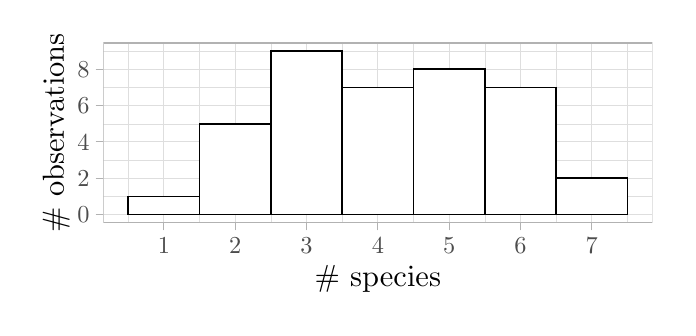
\begin{tikzpicture}[x=1pt,y=1pt]
\definecolor{fillColor}{RGB}{255,255,255}
\path[use as bounding box,fill=fillColor,fill opacity=0.00] (0,0) rectangle (231.26,101.18);
\begin{scope}
\path[clip] (  0.00,  0.00) rectangle (231.26,101.18);
\definecolor{drawColor}{RGB}{255,255,255}
\definecolor{fillColor}{RGB}{255,255,255}

\path[draw=drawColor,line width= 0.6pt,line join=round,line cap=round,fill=fillColor] (  0.00,  0.00) rectangle (231.26,101.18);
\end{scope}
\begin{scope}
\path[clip] ( 27.31, 30.69) rectangle (225.76, 95.68);
\definecolor{fillColor}{RGB}{255,255,255}

\path[fill=fillColor] ( 27.31, 30.69) rectangle (225.76, 95.68);
\definecolor{drawColor}{gray}{0.87}

\path[draw=drawColor,line width= 0.1pt,line join=round] ( 27.31, 40.20) --
	(225.76, 40.20);

\path[draw=drawColor,line width= 0.1pt,line join=round] ( 27.31, 53.33) --
	(225.76, 53.33);

\path[draw=drawColor,line width= 0.1pt,line join=round] ( 27.31, 66.46) --
	(225.76, 66.46);

\path[draw=drawColor,line width= 0.1pt,line join=round] ( 27.31, 79.59) --
	(225.76, 79.59);

\path[draw=drawColor,line width= 0.1pt,line join=round] ( 27.31, 92.72) --
	(225.76, 92.72);

\path[draw=drawColor,line width= 0.1pt,line join=round] ( 36.33, 30.69) --
	( 36.33, 95.68);

\path[draw=drawColor,line width= 0.1pt,line join=round] ( 62.11, 30.69) --
	( 62.11, 95.68);

\path[draw=drawColor,line width= 0.1pt,line join=round] ( 87.88, 30.69) --
	( 87.88, 95.68);

\path[draw=drawColor,line width= 0.1pt,line join=round] (113.65, 30.69) --
	(113.65, 95.68);

\path[draw=drawColor,line width= 0.1pt,line join=round] (139.43, 30.69) --
	(139.43, 95.68);

\path[draw=drawColor,line width= 0.1pt,line join=round] (165.20, 30.69) --
	(165.20, 95.68);

\path[draw=drawColor,line width= 0.1pt,line join=round] (190.97, 30.69) --
	(190.97, 95.68);

\path[draw=drawColor,line width= 0.1pt,line join=round] (216.74, 30.69) --
	(216.74, 95.68);

\path[draw=drawColor,line width= 0.3pt,line join=round] ( 27.31, 33.64) --
	(225.76, 33.64);

\path[draw=drawColor,line width= 0.3pt,line join=round] ( 27.31, 46.77) --
	(225.76, 46.77);

\path[draw=drawColor,line width= 0.3pt,line join=round] ( 27.31, 59.90) --
	(225.76, 59.90);

\path[draw=drawColor,line width= 0.3pt,line join=round] ( 27.31, 73.03) --
	(225.76, 73.03);

\path[draw=drawColor,line width= 0.3pt,line join=round] ( 27.31, 86.16) --
	(225.76, 86.16);

\path[draw=drawColor,line width= 0.3pt,line join=round] ( 49.22, 30.69) --
	( 49.22, 95.68);

\path[draw=drawColor,line width= 0.3pt,line join=round] ( 74.99, 30.69) --
	( 74.99, 95.68);

\path[draw=drawColor,line width= 0.3pt,line join=round] (100.77, 30.69) --
	(100.77, 95.68);

\path[draw=drawColor,line width= 0.3pt,line join=round] (126.54, 30.69) --
	(126.54, 95.68);

\path[draw=drawColor,line width= 0.3pt,line join=round] (152.31, 30.69) --
	(152.31, 95.68);

\path[draw=drawColor,line width= 0.3pt,line join=round] (178.08, 30.69) --
	(178.08, 95.68);

\path[draw=drawColor,line width= 0.3pt,line join=round] (203.86, 30.69) --
	(203.86, 95.68);
\definecolor{drawColor}{RGB}{0,0,0}

\path[draw=drawColor,line width= 0.6pt,line cap=rect,fill=fillColor] ( 36.33, 33.64) rectangle ( 62.11, 40.20);

\path[draw=drawColor,line width= 0.6pt,line cap=rect,fill=fillColor] ( 62.11, 33.64) rectangle ( 87.88, 66.46);

\path[draw=drawColor,line width= 0.6pt,line cap=rect,fill=fillColor] ( 87.88, 33.64) rectangle (113.65, 92.72);

\path[draw=drawColor,line width= 0.6pt,line cap=rect,fill=fillColor] (113.65, 33.64) rectangle (139.43, 79.59);

\path[draw=drawColor,line width= 0.6pt,line cap=rect,fill=fillColor] (139.43, 33.64) rectangle (165.20, 86.16);

\path[draw=drawColor,line width= 0.6pt,line cap=rect,fill=fillColor] (165.20, 33.64) rectangle (190.97, 79.59);

\path[draw=drawColor,line width= 0.6pt,line cap=rect,fill=fillColor] (190.97, 33.64) rectangle (216.74, 46.77);
\definecolor{drawColor}{gray}{0.70}

\path[draw=drawColor,line width= 0.6pt,line join=round,line cap=round] ( 27.31, 30.69) rectangle (225.76, 95.68);
\end{scope}
\begin{scope}
\path[clip] (  0.00,  0.00) rectangle (231.26,101.18);
\definecolor{drawColor}{gray}{0.30}

\node[text=drawColor,anchor=base east,inner sep=0pt, outer sep=0pt, scale=  0.88] at ( 22.36, 30.61) {0};

\node[text=drawColor,anchor=base east,inner sep=0pt, outer sep=0pt, scale=  0.88] at ( 22.36, 43.74) {2};

\node[text=drawColor,anchor=base east,inner sep=0pt, outer sep=0pt, scale=  0.88] at ( 22.36, 56.87) {4};

\node[text=drawColor,anchor=base east,inner sep=0pt, outer sep=0pt, scale=  0.88] at ( 22.36, 70.00) {6};

\node[text=drawColor,anchor=base east,inner sep=0pt, outer sep=0pt, scale=  0.88] at ( 22.36, 83.13) {8};
\end{scope}
\begin{scope}
\path[clip] (  0.00,  0.00) rectangle (231.26,101.18);
\definecolor{drawColor}{gray}{0.70}

\path[draw=drawColor,line width= 0.3pt,line join=round] ( 24.56, 33.64) --
	( 27.31, 33.64);

\path[draw=drawColor,line width= 0.3pt,line join=round] ( 24.56, 46.77) --
	( 27.31, 46.77);

\path[draw=drawColor,line width= 0.3pt,line join=round] ( 24.56, 59.90) --
	( 27.31, 59.90);

\path[draw=drawColor,line width= 0.3pt,line join=round] ( 24.56, 73.03) --
	( 27.31, 73.03);

\path[draw=drawColor,line width= 0.3pt,line join=round] ( 24.56, 86.16) --
	( 27.31, 86.16);
\end{scope}
\begin{scope}
\path[clip] (  0.00,  0.00) rectangle (231.26,101.18);
\definecolor{drawColor}{gray}{0.70}

\path[draw=drawColor,line width= 0.3pt,line join=round] ( 49.22, 27.94) --
	( 49.22, 30.69);

\path[draw=drawColor,line width= 0.3pt,line join=round] ( 74.99, 27.94) --
	( 74.99, 30.69);

\path[draw=drawColor,line width= 0.3pt,line join=round] (100.77, 27.94) --
	(100.77, 30.69);

\path[draw=drawColor,line width= 0.3pt,line join=round] (126.54, 27.94) --
	(126.54, 30.69);

\path[draw=drawColor,line width= 0.3pt,line join=round] (152.31, 27.94) --
	(152.31, 30.69);

\path[draw=drawColor,line width= 0.3pt,line join=round] (178.08, 27.94) --
	(178.08, 30.69);

\path[draw=drawColor,line width= 0.3pt,line join=round] (203.86, 27.94) --
	(203.86, 30.69);
\end{scope}
\begin{scope}
\path[clip] (  0.00,  0.00) rectangle (231.26,101.18);
\definecolor{drawColor}{gray}{0.30}

\node[text=drawColor,anchor=base,inner sep=0pt, outer sep=0pt, scale=  0.88] at ( 49.22, 19.68) {1};

\node[text=drawColor,anchor=base,inner sep=0pt, outer sep=0pt, scale=  0.88] at ( 74.99, 19.68) {2};

\node[text=drawColor,anchor=base,inner sep=0pt, outer sep=0pt, scale=  0.88] at (100.77, 19.68) {3};

\node[text=drawColor,anchor=base,inner sep=0pt, outer sep=0pt, scale=  0.88] at (126.54, 19.68) {4};

\node[text=drawColor,anchor=base,inner sep=0pt, outer sep=0pt, scale=  0.88] at (152.31, 19.68) {5};

\node[text=drawColor,anchor=base,inner sep=0pt, outer sep=0pt, scale=  0.88] at (178.08, 19.68) {6};

\node[text=drawColor,anchor=base,inner sep=0pt, outer sep=0pt, scale=  0.88] at (203.86, 19.68) {7};
\end{scope}
\begin{scope}
\path[clip] (  0.00,  0.00) rectangle (231.26,101.18);
\definecolor{drawColor}{RGB}{0,0,0}

\node[text=drawColor,anchor=base,inner sep=0pt, outer sep=0pt, scale=  1.10] at (126.54,  7.64) {\# species};
\end{scope}
\begin{scope}
\path[clip] (  0.00,  0.00) rectangle (231.26,101.18);
\definecolor{drawColor}{RGB}{0,0,0}

\node[text=drawColor,rotate= 90.00,anchor=base,inner sep=0pt, outer sep=0pt, scale=  1.10] at ( 13.08, 63.18) {\# observations};
\end{scope}
\end{tikzpicture}

    }
    \caption{Number of species in individual observations}
    \label{fig:nspeiciesDist}
\end{figure}

\begin{figure*}
    \centering
     \resizebox{\hsize}{!}{%
        % Created by tikzDevice version 0.12.3 on 2019-12-11 20:53:34
% !TEX encoding = UTF-8 Unicode
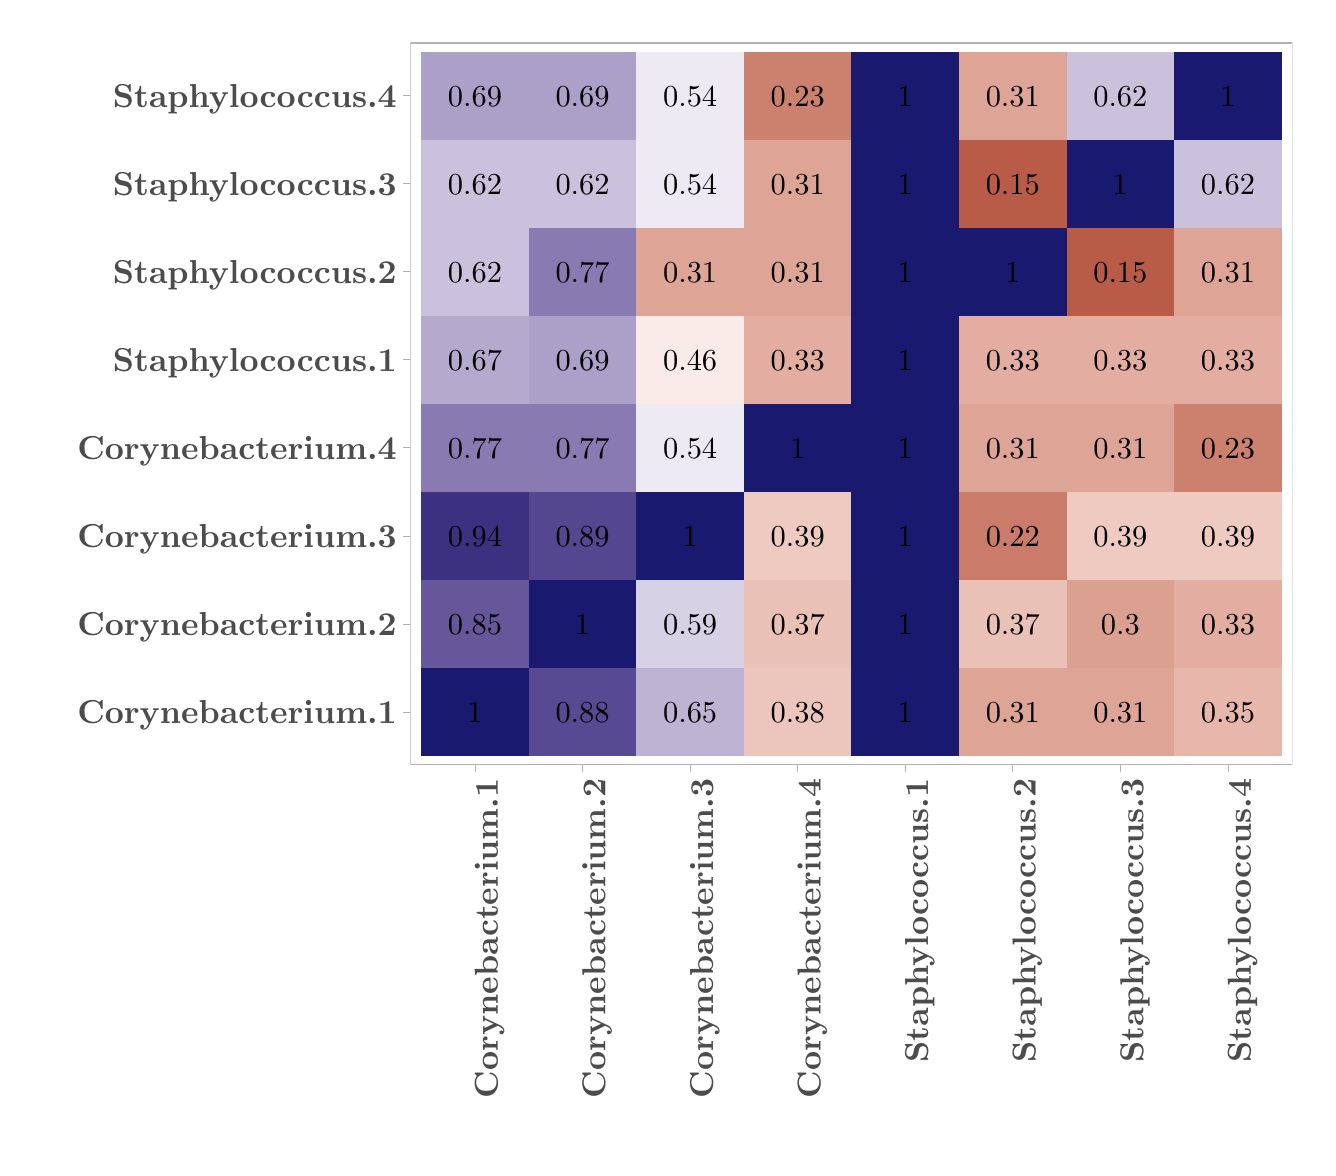
\begin{tikzpicture}[x=1pt,y=1pt]
\definecolor{fillColor}{RGB}{255,255,255}
\path[use as bounding box,fill=fillColor,fill opacity=0.00] (0,0) rectangle (462.53,404.71);
\begin{scope}
\path[clip] (  0.00,  0.00) rectangle (462.53,404.71);
\definecolor{drawColor}{RGB}{255,255,255}
\definecolor{fillColor}{RGB}{255,255,255}

\path[draw=drawColor,line width= 0.6pt,line join=round,line cap=round,fill=fillColor] (  0.00,  0.00) rectangle (462.53,404.71);
\end{scope}
\begin{scope}
\path[clip] (138.33,138.33) rectangle (457.03,399.21);
\definecolor{fillColor}{RGB}{255,255,255}

\path[fill=fillColor] (138.33,138.33) rectangle (457.03,399.21);
\definecolor{fillColor}{RGB}{25,25,112}

\path[fill=fillColor] (142.21,141.51) rectangle (181.08,173.32);
\definecolor{fillColor}{RGB}{88,74,146}

\path[fill=fillColor] (181.08,141.51) rectangle (219.95,173.32);
\definecolor{fillColor}{RGB}{189,179,211}

\path[fill=fillColor] (219.95,141.51) rectangle (258.81,173.32);
\definecolor{fillColor}{RGB}{236,198,188}

\path[fill=fillColor] (258.81,141.51) rectangle (297.68,173.32);
\definecolor{fillColor}{RGB}{25,25,112}

\path[fill=fillColor] (297.68,141.51) rectangle (336.54,173.32);
\definecolor{fillColor}{RGB}{222,165,151}

\path[fill=fillColor] (336.54,141.51) rectangle (375.41,173.32);

\path[fill=fillColor] (375.41,141.51) rectangle (414.28,173.32);
\definecolor{fillColor}{RGB}{231,183,172}

\path[fill=fillColor] (414.28,141.51) rectangle (453.14,173.32);
\definecolor{fillColor}{RGB}{102,87,154}

\path[fill=fillColor] (142.21,173.32) rectangle (181.08,205.14);
\definecolor{fillColor}{RGB}{25,25,112}

\path[fill=fillColor] (181.08,173.32) rectangle (219.95,205.14);
\definecolor{fillColor}{RGB}{215,209,229}

\path[fill=fillColor] (219.95,173.32) rectangle (258.81,205.14);
\definecolor{fillColor}{RGB}{234,193,183}

\path[fill=fillColor] (258.81,173.32) rectangle (297.68,205.14);
\definecolor{fillColor}{RGB}{25,25,112}

\path[fill=fillColor] (297.68,173.32) rectangle (336.54,205.14);
\definecolor{fillColor}{RGB}{234,193,183}

\path[fill=fillColor] (336.54,173.32) rectangle (375.41,205.14);
\definecolor{fillColor}{RGB}{220,160,145}

\path[fill=fillColor] (375.41,173.32) rectangle (414.28,205.14);
\definecolor{fillColor}{RGB}{227,174,161}

\path[fill=fillColor] (414.28,173.32) rectangle (453.14,205.14);
\definecolor{fillColor}{RGB}{60,49,129}

\path[fill=fillColor] (142.21,205.14) rectangle (181.08,236.95);
\definecolor{fillColor}{RGB}{84,70,143}

\path[fill=fillColor] (181.08,205.14) rectangle (219.95,236.95);
\definecolor{fillColor}{RGB}{25,25,112}

\path[fill=fillColor] (219.95,205.14) rectangle (258.81,236.95);
\definecolor{fillColor}{RGB}{238,202,193}

\path[fill=fillColor] (258.81,205.14) rectangle (297.68,236.95);
\definecolor{fillColor}{RGB}{25,25,112}

\path[fill=fillColor] (297.68,205.14) rectangle (336.54,236.95);
\definecolor{fillColor}{RGB}{202,123,105}

\path[fill=fillColor] (336.54,205.14) rectangle (375.41,236.95);
\definecolor{fillColor}{RGB}{238,202,193}

\path[fill=fillColor] (375.41,205.14) rectangle (414.28,236.95);

\path[fill=fillColor] (414.28,205.14) rectangle (453.14,236.95);
\definecolor{fillColor}{RGB}{137,123,177}

\path[fill=fillColor] (142.21,236.95) rectangle (181.08,268.77);

\path[fill=fillColor] (181.08,236.95) rectangle (219.95,268.77);
\definecolor{fillColor}{RGB}{237,234,243}

\path[fill=fillColor] (219.95,236.95) rectangle (258.81,268.77);
\definecolor{fillColor}{RGB}{25,25,112}

\path[fill=fillColor] (258.81,236.95) rectangle (297.68,268.77);

\path[fill=fillColor] (297.68,236.95) rectangle (336.54,268.77);
\definecolor{fillColor}{RGB}{222,165,151}

\path[fill=fillColor] (336.54,236.95) rectangle (375.41,268.77);

\path[fill=fillColor] (375.41,236.95) rectangle (414.28,268.77);
\definecolor{fillColor}{RGB}{204,128,110}

\path[fill=fillColor] (414.28,236.95) rectangle (453.14,268.77);
\definecolor{fillColor}{RGB}{180,170,206}

\path[fill=fillColor] (142.21,268.77) rectangle (181.08,300.58);
\definecolor{fillColor}{RGB}{171,160,200}

\path[fill=fillColor] (181.08,268.77) rectangle (219.95,300.58);
\definecolor{fillColor}{RGB}{249,236,232}

\path[fill=fillColor] (219.95,268.77) rectangle (258.81,300.58);
\definecolor{fillColor}{RGB}{227,174,161}

\path[fill=fillColor] (258.81,268.77) rectangle (297.68,300.58);
\definecolor{fillColor}{RGB}{25,25,112}

\path[fill=fillColor] (297.68,268.77) rectangle (336.54,300.58);
\definecolor{fillColor}{RGB}{227,174,161}

\path[fill=fillColor] (336.54,268.77) rectangle (375.41,300.58);

\path[fill=fillColor] (375.41,268.77) rectangle (414.28,300.58);

\path[fill=fillColor] (414.28,268.77) rectangle (453.14,300.58);
\definecolor{fillColor}{RGB}{202,194,220}

\path[fill=fillColor] (142.21,300.58) rectangle (181.08,332.40);
\definecolor{fillColor}{RGB}{137,123,177}

\path[fill=fillColor] (181.08,300.58) rectangle (219.95,332.40);
\definecolor{fillColor}{RGB}{222,165,151}

\path[fill=fillColor] (219.95,300.58) rectangle (258.81,332.40);

\path[fill=fillColor] (258.81,300.58) rectangle (297.68,332.40);
\definecolor{fillColor}{RGB}{25,25,112}

\path[fill=fillColor] (297.68,300.58) rectangle (336.54,332.40);

\path[fill=fillColor] (336.54,300.58) rectangle (375.41,332.40);
\definecolor{fillColor}{RGB}{184,91,71}

\path[fill=fillColor] (375.41,300.58) rectangle (414.28,332.40);
\definecolor{fillColor}{RGB}{222,165,151}

\path[fill=fillColor] (414.28,300.58) rectangle (453.14,332.40);
\definecolor{fillColor}{RGB}{202,194,220}

\path[fill=fillColor] (142.21,332.40) rectangle (181.08,364.22);

\path[fill=fillColor] (181.08,332.40) rectangle (219.95,364.22);
\definecolor{fillColor}{RGB}{237,234,243}

\path[fill=fillColor] (219.95,332.40) rectangle (258.81,364.22);
\definecolor{fillColor}{RGB}{222,165,151}

\path[fill=fillColor] (258.81,332.40) rectangle (297.68,364.22);
\definecolor{fillColor}{RGB}{25,25,112}

\path[fill=fillColor] (297.68,332.40) rectangle (336.54,364.22);
\definecolor{fillColor}{RGB}{184,91,71}

\path[fill=fillColor] (336.54,332.40) rectangle (375.41,364.22);
\definecolor{fillColor}{RGB}{25,25,112}

\path[fill=fillColor] (375.41,332.40) rectangle (414.28,364.22);
\definecolor{fillColor}{RGB}{202,194,220}

\path[fill=fillColor] (414.28,332.40) rectangle (453.14,364.22);
\definecolor{fillColor}{RGB}{171,160,200}

\path[fill=fillColor] (142.21,364.22) rectangle (181.08,396.03);

\path[fill=fillColor] (181.08,364.22) rectangle (219.95,396.03);
\definecolor{fillColor}{RGB}{237,234,243}

\path[fill=fillColor] (219.95,364.22) rectangle (258.81,396.03);
\definecolor{fillColor}{RGB}{204,128,110}

\path[fill=fillColor] (258.81,364.22) rectangle (297.68,396.03);
\definecolor{fillColor}{RGB}{25,25,112}

\path[fill=fillColor] (297.68,364.22) rectangle (336.54,396.03);
\definecolor{fillColor}{RGB}{222,165,151}

\path[fill=fillColor] (336.54,364.22) rectangle (375.41,396.03);
\definecolor{fillColor}{RGB}{202,194,220}

\path[fill=fillColor] (375.41,364.22) rectangle (414.28,396.03);
\definecolor{fillColor}{RGB}{25,25,112}

\path[fill=fillColor] (414.28,364.22) rectangle (453.14,396.03);
\definecolor{drawColor}{RGB}{0,0,0}

\node[text=drawColor,anchor=base,inner sep=0pt, outer sep=0pt, scale=  1.10] at (161.65,153.61) {1};

\node[text=drawColor,anchor=base,inner sep=0pt, outer sep=0pt, scale=  1.10] at (200.51,153.61) {0.88};

\node[text=drawColor,anchor=base,inner sep=0pt, outer sep=0pt, scale=  1.10] at (239.38,153.61) {0.65};

\node[text=drawColor,anchor=base,inner sep=0pt, outer sep=0pt, scale=  1.10] at (278.24,153.61) {0.38};

\node[text=drawColor,anchor=base,inner sep=0pt, outer sep=0pt, scale=  1.10] at (317.11,153.61) {1};

\node[text=drawColor,anchor=base,inner sep=0pt, outer sep=0pt, scale=  1.10] at (355.98,153.61) {0.31};

\node[text=drawColor,anchor=base,inner sep=0pt, outer sep=0pt, scale=  1.10] at (394.84,153.61) {0.31};

\node[text=drawColor,anchor=base,inner sep=0pt, outer sep=0pt, scale=  1.10] at (433.71,153.61) {0.35};

\node[text=drawColor,anchor=base,inner sep=0pt, outer sep=0pt, scale=  1.10] at (161.65,185.43) {0.85};

\node[text=drawColor,anchor=base,inner sep=0pt, outer sep=0pt, scale=  1.10] at (200.51,185.43) {1};

\node[text=drawColor,anchor=base,inner sep=0pt, outer sep=0pt, scale=  1.10] at (239.38,185.43) {0.59};

\node[text=drawColor,anchor=base,inner sep=0pt, outer sep=0pt, scale=  1.10] at (278.24,185.43) {0.37};

\node[text=drawColor,anchor=base,inner sep=0pt, outer sep=0pt, scale=  1.10] at (317.11,185.43) {1};

\node[text=drawColor,anchor=base,inner sep=0pt, outer sep=0pt, scale=  1.10] at (355.98,185.43) {0.37};

\node[text=drawColor,anchor=base,inner sep=0pt, outer sep=0pt, scale=  1.10] at (394.84,185.43) {0.3};

\node[text=drawColor,anchor=base,inner sep=0pt, outer sep=0pt, scale=  1.10] at (433.71,185.43) {0.33};

\node[text=drawColor,anchor=base,inner sep=0pt, outer sep=0pt, scale=  1.10] at (161.65,217.25) {0.94};

\node[text=drawColor,anchor=base,inner sep=0pt, outer sep=0pt, scale=  1.10] at (200.51,217.25) {0.89};

\node[text=drawColor,anchor=base,inner sep=0pt, outer sep=0pt, scale=  1.10] at (239.38,217.25) {1};

\node[text=drawColor,anchor=base,inner sep=0pt, outer sep=0pt, scale=  1.10] at (278.24,217.25) {0.39};

\node[text=drawColor,anchor=base,inner sep=0pt, outer sep=0pt, scale=  1.10] at (317.11,217.25) {1};

\node[text=drawColor,anchor=base,inner sep=0pt, outer sep=0pt, scale=  1.10] at (355.98,217.25) {0.22};

\node[text=drawColor,anchor=base,inner sep=0pt, outer sep=0pt, scale=  1.10] at (394.84,217.25) {0.39};

\node[text=drawColor,anchor=base,inner sep=0pt, outer sep=0pt, scale=  1.10] at (433.71,217.25) {0.39};

\node[text=drawColor,anchor=base,inner sep=0pt, outer sep=0pt, scale=  1.10] at (161.65,249.06) {0.77};

\node[text=drawColor,anchor=base,inner sep=0pt, outer sep=0pt, scale=  1.10] at (200.51,249.06) {0.77};

\node[text=drawColor,anchor=base,inner sep=0pt, outer sep=0pt, scale=  1.10] at (239.38,249.06) {0.54};

\node[text=drawColor,anchor=base,inner sep=0pt, outer sep=0pt, scale=  1.10] at (278.24,249.06) {1};

\node[text=drawColor,anchor=base,inner sep=0pt, outer sep=0pt, scale=  1.10] at (317.11,249.06) {1};

\node[text=drawColor,anchor=base,inner sep=0pt, outer sep=0pt, scale=  1.10] at (355.98,249.06) {0.31};

\node[text=drawColor,anchor=base,inner sep=0pt, outer sep=0pt, scale=  1.10] at (394.84,249.06) {0.31};

\node[text=drawColor,anchor=base,inner sep=0pt, outer sep=0pt, scale=  1.10] at (433.71,249.06) {0.23};

\node[text=drawColor,anchor=base,inner sep=0pt, outer sep=0pt, scale=  1.10] at (161.65,280.88) {0.67};

\node[text=drawColor,anchor=base,inner sep=0pt, outer sep=0pt, scale=  1.10] at (200.51,280.88) {0.69};

\node[text=drawColor,anchor=base,inner sep=0pt, outer sep=0pt, scale=  1.10] at (239.38,280.88) {0.46};

\node[text=drawColor,anchor=base,inner sep=0pt, outer sep=0pt, scale=  1.10] at (278.24,280.88) {0.33};

\node[text=drawColor,anchor=base,inner sep=0pt, outer sep=0pt, scale=  1.10] at (317.11,280.88) {1};

\node[text=drawColor,anchor=base,inner sep=0pt, outer sep=0pt, scale=  1.10] at (355.98,280.88) {0.33};

\node[text=drawColor,anchor=base,inner sep=0pt, outer sep=0pt, scale=  1.10] at (394.84,280.88) {0.33};

\node[text=drawColor,anchor=base,inner sep=0pt, outer sep=0pt, scale=  1.10] at (433.71,280.88) {0.33};

\node[text=drawColor,anchor=base,inner sep=0pt, outer sep=0pt, scale=  1.10] at (161.65,312.69) {0.62};

\node[text=drawColor,anchor=base,inner sep=0pt, outer sep=0pt, scale=  1.10] at (200.51,312.69) {0.77};

\node[text=drawColor,anchor=base,inner sep=0pt, outer sep=0pt, scale=  1.10] at (239.38,312.69) {0.31};

\node[text=drawColor,anchor=base,inner sep=0pt, outer sep=0pt, scale=  1.10] at (278.24,312.69) {0.31};

\node[text=drawColor,anchor=base,inner sep=0pt, outer sep=0pt, scale=  1.10] at (317.11,312.69) {1};

\node[text=drawColor,anchor=base,inner sep=0pt, outer sep=0pt, scale=  1.10] at (355.98,312.69) {1};

\node[text=drawColor,anchor=base,inner sep=0pt, outer sep=0pt, scale=  1.10] at (394.84,312.69) {0.15};

\node[text=drawColor,anchor=base,inner sep=0pt, outer sep=0pt, scale=  1.10] at (433.71,312.69) {0.31};

\node[text=drawColor,anchor=base,inner sep=0pt, outer sep=0pt, scale=  1.10] at (161.65,344.51) {0.62};

\node[text=drawColor,anchor=base,inner sep=0pt, outer sep=0pt, scale=  1.10] at (200.51,344.51) {0.62};

\node[text=drawColor,anchor=base,inner sep=0pt, outer sep=0pt, scale=  1.10] at (239.38,344.51) {0.54};

\node[text=drawColor,anchor=base,inner sep=0pt, outer sep=0pt, scale=  1.10] at (278.24,344.51) {0.31};

\node[text=drawColor,anchor=base,inner sep=0pt, outer sep=0pt, scale=  1.10] at (317.11,344.51) {1};

\node[text=drawColor,anchor=base,inner sep=0pt, outer sep=0pt, scale=  1.10] at (355.98,344.51) {0.15};

\node[text=drawColor,anchor=base,inner sep=0pt, outer sep=0pt, scale=  1.10] at (394.84,344.51) {1};

\node[text=drawColor,anchor=base,inner sep=0pt, outer sep=0pt, scale=  1.10] at (433.71,344.51) {0.62};

\node[text=drawColor,anchor=base,inner sep=0pt, outer sep=0pt, scale=  1.10] at (161.65,376.32) {0.69};

\node[text=drawColor,anchor=base,inner sep=0pt, outer sep=0pt, scale=  1.10] at (200.51,376.32) {0.69};

\node[text=drawColor,anchor=base,inner sep=0pt, outer sep=0pt, scale=  1.10] at (239.38,376.32) {0.54};

\node[text=drawColor,anchor=base,inner sep=0pt, outer sep=0pt, scale=  1.10] at (278.24,376.32) {0.23};

\node[text=drawColor,anchor=base,inner sep=0pt, outer sep=0pt, scale=  1.10] at (317.11,376.32) {1};

\node[text=drawColor,anchor=base,inner sep=0pt, outer sep=0pt, scale=  1.10] at (355.98,376.32) {0.31};

\node[text=drawColor,anchor=base,inner sep=0pt, outer sep=0pt, scale=  1.10] at (394.84,376.32) {0.62};

\node[text=drawColor,anchor=base,inner sep=0pt, outer sep=0pt, scale=  1.10] at (433.71,376.32) {1};
\definecolor{drawColor}{gray}{0.70}

\path[draw=drawColor,line width= 0.6pt,line join=round,line cap=round] (138.33,138.33) rectangle (457.03,399.21);
\end{scope}
\begin{scope}
\path[clip] (  0.00,  0.00) rectangle (462.53,404.71);
\definecolor{drawColor}{gray}{0.30}

\node[text=drawColor,anchor=base east,inner sep=0pt, outer sep=0pt, scale=  1.20] at (133.38,153.28) {\bfseries Corynebacterium.1};

\node[text=drawColor,anchor=base east,inner sep=0pt, outer sep=0pt, scale=  1.20] at (133.38,185.09) {\bfseries Corynebacterium.2};

\node[text=drawColor,anchor=base east,inner sep=0pt, outer sep=0pt, scale=  1.20] at (133.38,216.91) {\bfseries Corynebacterium.3};

\node[text=drawColor,anchor=base east,inner sep=0pt, outer sep=0pt, scale=  1.20] at (133.38,248.72) {\bfseries Corynebacterium.4};

\node[text=drawColor,anchor=base east,inner sep=0pt, outer sep=0pt, scale=  1.20] at (133.38,280.54) {\bfseries Staphylococcus.1};

\node[text=drawColor,anchor=base east,inner sep=0pt, outer sep=0pt, scale=  1.20] at (133.38,312.35) {\bfseries Staphylococcus.2};

\node[text=drawColor,anchor=base east,inner sep=0pt, outer sep=0pt, scale=  1.20] at (133.38,344.17) {\bfseries Staphylococcus.3};

\node[text=drawColor,anchor=base east,inner sep=0pt, outer sep=0pt, scale=  1.20] at (133.38,375.98) {\bfseries Staphylococcus.4};
\end{scope}
\begin{scope}
\path[clip] (  0.00,  0.00) rectangle (462.53,404.71);
\definecolor{drawColor}{gray}{0.70}

\path[draw=drawColor,line width= 0.3pt,line join=round] (135.58,157.42) --
	(138.33,157.42);

\path[draw=drawColor,line width= 0.3pt,line join=round] (135.58,189.23) --
	(138.33,189.23);

\path[draw=drawColor,line width= 0.3pt,line join=round] (135.58,221.05) --
	(138.33,221.05);

\path[draw=drawColor,line width= 0.3pt,line join=round] (135.58,252.86) --
	(138.33,252.86);

\path[draw=drawColor,line width= 0.3pt,line join=round] (135.58,284.68) --
	(138.33,284.68);

\path[draw=drawColor,line width= 0.3pt,line join=round] (135.58,316.49) --
	(138.33,316.49);

\path[draw=drawColor,line width= 0.3pt,line join=round] (135.58,348.31) --
	(138.33,348.31);

\path[draw=drawColor,line width= 0.3pt,line join=round] (135.58,380.12) --
	(138.33,380.12);
\end{scope}
\begin{scope}
\path[clip] (  0.00,  0.00) rectangle (462.53,404.71);
\definecolor{drawColor}{gray}{0.70}

\path[draw=drawColor,line width= 0.3pt,line join=round] (161.65,135.58) --
	(161.65,138.33);

\path[draw=drawColor,line width= 0.3pt,line join=round] (200.51,135.58) --
	(200.51,138.33);

\path[draw=drawColor,line width= 0.3pt,line join=round] (239.38,135.58) --
	(239.38,138.33);

\path[draw=drawColor,line width= 0.3pt,line join=round] (278.24,135.58) --
	(278.24,138.33);

\path[draw=drawColor,line width= 0.3pt,line join=round] (317.11,135.58) --
	(317.11,138.33);

\path[draw=drawColor,line width= 0.3pt,line join=round] (355.98,135.58) --
	(355.98,138.33);

\path[draw=drawColor,line width= 0.3pt,line join=round] (394.84,135.58) --
	(394.84,138.33);

\path[draw=drawColor,line width= 0.3pt,line join=round] (433.71,135.58) --
	(433.71,138.33);
\end{scope}
\begin{scope}
\path[clip] (  0.00,  0.00) rectangle (462.53,404.71);
\definecolor{drawColor}{gray}{0.30}

\node[text=drawColor,rotate= 90.00,anchor=base east,inner sep=0pt, outer sep=0pt, scale=  1.20] at (169.93,133.38) {\bfseries Corynebacterium.1};

\node[text=drawColor,rotate= 90.00,anchor=base east,inner sep=0pt, outer sep=0pt, scale=  1.20] at (208.79,133.38) {\bfseries Corynebacterium.2};

\node[text=drawColor,rotate= 90.00,anchor=base east,inner sep=0pt, outer sep=0pt, scale=  1.20] at (247.66,133.38) {\bfseries Corynebacterium.3};

\node[text=drawColor,rotate= 90.00,anchor=base east,inner sep=0pt, outer sep=0pt, scale=  1.20] at (286.53,133.38) {\bfseries Corynebacterium.4};

\node[text=drawColor,rotate= 90.00,anchor=base east,inner sep=0pt, outer sep=0pt, scale=  1.20] at (325.39,133.38) {\bfseries Staphylococcus.1};

\node[text=drawColor,rotate= 90.00,anchor=base east,inner sep=0pt, outer sep=0pt, scale=  1.20] at (364.26,133.38) {\bfseries Staphylococcus.2};

\node[text=drawColor,rotate= 90.00,anchor=base east,inner sep=0pt, outer sep=0pt, scale=  1.20] at (403.12,133.38) {\bfseries Staphylococcus.3};

\node[text=drawColor,rotate= 90.00,anchor=base east,inner sep=0pt, outer sep=0pt, scale=  1.20] at (441.99,133.38) {\bfseries Staphylococcus.4};
\end{scope}
\end{tikzpicture}

    }
    \caption{conditional Probability of joint occurance}
    \label{fig:conditionalPjointoccurance}
\end{figure*}